\documentclass[a4paper,11pt]{article}
\usepackage{graphicx}
\usepackage{subfigure}
\usepackage{geometry}
\usepackage{framed}
\usepackage{lipsum}
\usepackage{color}
\usepackage{amsmath}
\usepackage{amssymb}
\usepackage{amsthm}
\usepackage{multirow}
\usepackage{titlesec}
\usepackage{enumerate}
\usepackage{mathrsfs}
\usepackage{ctex}


% 定义各种环境
\newtheorem{theorem}{Theorem}[section]
\newtheorem{lemma}[theorem]{Lemma}
\newtheorem{corollary}[theorem]{Corollary}
\newtheorem{proposition}[theorem]{Proposition}
\newtheorem{example}[theorem]{Example}
\theoremstyle{definition}
\newtheorem{remark}[theorem]{Remark}
\newtheorem{definition}[theorem]{Definition}
\newtheorem{assumption}[theorem]{Assumption}

\def \supp {\mathop\mathrm{\,supp\,}}
\def \sgn{\mathrm{\,sgn\,}}
\def \esssup {\mathop\mathrm{\,esssup\,}}

% 设置 proof 的格式
% \renewcommand{\proofname}{\emph{Proof}}

% 基本信息
\title{笔记-J. Duoandikoetxea, Fourier Analysis}

\begin{document}


\maketitle

\section{待整理}

\begin{lemma} \label{h2}
    设 $ N \in \mathbb{N} $, 开区间 $ \{I_k\}_{k = 1}^N \subset \mathbb{R} $ 且
    $$
        \bigcap_{k = 1}^N I_k \neq \emptyset.
    $$
    则存在 $ k_0 \in \{1, \ldots, N\} $ 使得
    $$
        \bigcup_{k = 1}^N I_k = I_{k_0},
    $$
    或存在 $ k_1, k_2 \in \{1, \ldots, N\} $ 使得
    $$
        \bigcup_{k = 1}^N I_k = I_{k_1} \cup I_{k_2}.
    $$
\end{lemma}

\begin{proof}
    若存在 $ k_0 \in \{1, \ldots, N\} $ 使得
    $$
        \bigcup_{k = 1}^N I_k = I_{k_0},
    $$
    Lemma \ref{h2} 证毕. 
    否则由 $ \bigcap_{k = 1}^N I_k \neq \emptyset $ 知, 
    存在 $ a, b \in \mathbb{R} $, $ a < b $ 使得
    $$
        \bigcup_{\alpha \in A} I_k = (a, b).
    $$
    存在 $ k_1, k_2 \in \{1, \ldots, N\} $ 使得
    $$
        \inf I_{k_1} = a, \quad \text{and} \quad \sup I_{k_2} = b.
    $$
    由此及 $ I_{k_1} \cap I_{k_2} \neq \emptyset $ 知
    $$
        \bigcup_{k = 1}^N I_k = I_{k_1} \cup I_{k_2}.
    $$
\end{proof}

\begin{lemma}[Lemma 2.6]
    Let $ \{ I_\alpha \}_{\alpha \in A} $ be a collection of open intervals in $ \mathbb{R}^n $ 
    and let $ K $ be a compact set contained in their union. Then there exists a finite subcollection
    $ \{ I_j \} $ such that
    $$
        K \subset \bigcup_j I_j, \quad \text{and} \quad 
        \forall x \in \mathbb{R},\ \sum_j \mathrm{1}_{I_j} (x) \leq 2.
    $$
\end{lemma}

\begin{proof}
    由 $ K $ 是紧集知, 存在 $ \{I_k^{(0)}\}_{k = 1}^{N_0} \subset \{ I_\alpha \}_{\alpha \in A} $ 使得
    $$
        K \subset \bigcup_{k = 1}^N I_k^{(0)}.
    $$
    若存在 $ x_0 \in \mathbb{R} $ 使得 $ \sum_{k = 1}^{N_0} \mathrm{1}_{I_j^{(0)}} (x_0) \geq 3 $, 
    则由 Lemma \ref{lem1} 知,
    存在 $ \{I_k^{(1)}\}_{k = 1}^{N_1} \subset \{ I_\alpha \}_{\alpha \in A} $ 使得 $ N_1 \leq N_0 - 1 $ 且
    $$
        K \subset \bigcup_{k = 1}^{N_1} I_k^{(1)}.
    $$
    若存在 $ x_1 \in \mathbb{R} $ 使得 $ \sum_{k = 1}^{N_1} \mathrm{1}_{I_j^{(1)}} (x_1) \geq 3 $, 重复之前的过程.
    由于 $ \{N_k\} $ 严格减且大于 $ 0 $,
    故此过程经过有限次后会停止, 此时存在 $ \{I_k^{(s)}\}_{k = 1}^{N_s} \subset \{ I_\alpha \}_{\alpha \in A} $ 使得
    $$
        K \subset \bigcup_{k = 1}^{N_s} I_k^{(s)} \quad \text{and} \quad 
        \forall x \in \mathbb{R},\ \sum_{k = 1}^{N_s} \mathrm{1}_{I_k^{(s)}} (x) \leq 2.
    $$
\end{proof}

Lemma 2.12 的证明中会用到如下事实.

\begin{theorem}
    设方体 $ Q_1, Q_2 $ 满足 $ Q_1 \subset Q_2 $, 
    则对 $ \forall \alpha \in [1, \infty) $, 
    $ \alpha Q_1 \subset \alpha Q_2 $. 其中 $ \alpha Q_1 $ 表示与 $ Q_1 $ 中心相同, 长度为 $ \alpha \ell(Q_1) $ 的方体.
\end{theorem}

\begin{proof}
    由 $ Q_1 \subset Q_2 $ 知, $ \ell(Q_1) \leq \ell(Q_2) $, 因此
    对 $ \forall x := (x_1, \ldots, x_n) \in \alpha Q_1 $, $ \forall k \in \{1, \ldots, n\} $,
    \begin{align*}
        |x_k - (x_{Q_2})_k| 
            &\leq |x_k - (x_{Q_1})_k| + |(x_{Q_1})_k - (x_{Q_2})_k| \\
            &\leq \frac{\alpha \ell(Q_1)}{2} + \frac{\ell(Q_2) - \ell(Q_1)}{2} \\
            &= \frac{(\alpha - 1) \ell(Q_1)}{2} + \frac{\ell(Q_2)}{2}
            \leq \frac{\alpha \ell(Q_2)}{2}.
    \end{align*}
    因此 $ x \in \alpha Q_2 $.
\end{proof}

\section*{3.4 Truncated integrals and pointwise convergence}

\begin{framed}
    For $ \varepsilon > 0 $, the functions $ y^{-1} \mathbf{1}_{\{|y| > \varepsilon\}} $  
    belong to $ L^q(\mathbb{R}) $, $ 1 < q \leq \infty $, so the functions
    $$
        H_\varepsilon (f) (x) 
            := \frac{1}{\pi} \int_{|y| > \varepsilon} \frac{f(x - y)}{y} \, dy 
    $$
    are well defined if $ f \in L^p(\mathbb{R}) $, $ p \in [1, \infty) $.
\end{framed}

在以下全文中, 对 $ \forall \varepsilon \in (0, \infty) $, $ \forall y \in \mathbb{R} $, 令
$ \psi := y^{-1} \mathbf{1}_{\{y \in \mathbb{R} :\ |y| > 1\}} $, 
$$
    \psi_\varepsilon(y) := \frac{1}{\varepsilon} \psi \left( \frac{y}{\varepsilon} \right) 
        = \left\{ \begin{aligned}
        &\frac{1}{y}, && |y| > \varepsilon, \\
        &0,           && |y| \leq \varepsilon.
    \end{aligned} \right.
$$
设 $ \varepsilon \in (0, \infty) $, $ p \in [1, \infty) $. 则
对 $ \forall f \in L^p(\mathbb{R}) $, $ \forall x \in \mathbb{R} $,
$$
    H_\varepsilon (f) (x) 
        = \frac{1}{\pi} \int_{\{y \in \mathbb{R}:\ |y| > \varepsilon\}} \frac{f(x - y)}{y} \, dy  
        = \frac{1}{\pi} \int_\mathbb{R} f(x - y) \psi_\varepsilon(y) \, dy 
        = \frac{1}{\pi} (f * \psi_\varepsilon)(x),
$$
即在点点意义下
$$
    H_\varepsilon (f) = \frac{1}{\pi} (f * \psi_\varepsilon).
$$

\begin{remark} \label{remark1}
    设 $ \varepsilon \in (0, \infty) $. 
    \begin{enumerate}[(i)]
      \item 对 $ q \in (1, \infty] $, 
        $ \psi_\varepsilon \in L^q(\mathbb{R}) $;
      \item 若 $ f \in L^1(\mathbb{R}) $, 则对 $ \forall q \in (1, \infty] $, 
        $ H_\varepsilon (f) \in L^q(\mathbb{R}) $.
    \end{enumerate}
\end{remark} 

\begin{proof}
    先证 (i). 当 $ q = \infty $ 时,
    $$
        \| \psi_\varepsilon \|_{L^q(\mathbb{R})}
            = \esssup_{y \in \mathbb{R}} | \psi_\varepsilon(y) |
            = \sup_{y \in \mathbb{R}, |y| > \varepsilon} \left| \frac{1}{y} \right|
            = \frac{1}{\varepsilon} < \infty.
    $$
    当 $ q \in (1, \infty) $ 时,
    $$
        \| \psi_\varepsilon \|_{L^q(\mathbb{R})}
            = \left[ \int_\mathbb{R} |\psi_\varepsilon(y)|^q \, dy \right]^{1/q}
            = \left( 2 \int_\varepsilon^\infty \frac{1}{y^q} \, dy \right)^{1/q}  
            = \left( \frac{2 \varepsilon^{1 - q}}{q - 1} \right)^{1/q}  
            < \infty.
    $$
    因此对 $ \forall q \in (1, \infty] $, $ \psi_\varepsilon \in L^q(\mathbb{R}) $.
    
    再证 (ii). 对 $ \forall q \in (1, \infty] $, 
    由 (i) 知 $ \psi_\varepsilon \in L^q(\mathbb{R}) $.
    由此, $ f \in L^1(\mathbb{R}) $ 和 Young 不等式([丁勇, 定理 1.1.2]) 知,
    $$
        H_\varepsilon (f)
            = \frac{1}{\pi} (f * \psi_\varepsilon)
            \in L^q(\mathbb{R}).
    $$
    注 \ref{remark1} 证毕.
\end{proof}
  
\begin{remark} 
    设 $ p \in [1, \infty) $ 且 $ f \in L^p(\mathbb{R}) $. 则 $ H_\varepsilon (f) $ 是良定义的.
\end{remark}

\begin{proof}
    由 H\"older 不等式知, $ \forall x \in \mathbb{R} $,
    $$
        \int_\mathbb{R} | f(x - y) \psi_\varepsilon(y) | \, dy
            \overset{\text{H\"older 不等式}}{\leq} 
            \| f \|_{L^p(\mathbb{R})} \| \psi_\varepsilon \|_{L^{p'}(\mathbb{R})} < \infty.
    $$
    因此 $ H_\varepsilon (f) $ 是良定义的.
\end{proof}


\begin{framed}
    Moreover, $ H_\varepsilon $ satisfies weak $ (1, 1) $ and
    strong $ (p, p) $ estimates like those in Theorem 3.2 with constants that are
    uniformly bounded for all $ \varepsilon $.
    To see this, we first note that 
    $$ 
        \left( \frac{1}{y} \mathbf{1}_{\{|y| > \varepsilon\}} \right)^\wedge (\xi)
            = - 2 i \sgn (\xi) \lim_{N \to \infty} 
                \int_{2 \pi \varepsilon |\xi|}^{2 \pi N |\xi|} \frac{\sin (t)}{t} \, dt.
    $$ 
    This is uniformly bounded,
    so the strong $ (2,2) $ inequality holds with constant independent of $ \varepsilon $.
\end{framed}

\begin{lemma} \label{lem4}
    可测函数列 $ \{f_k\}_{k \in \mathbb{N}} $ 依测度收敛到 $ f $
    且几乎处处收敛到 $ g $. 则对 几乎处处 $ x \in \mathbb{R} $, $ f(x) = g(x) $.
\end{lemma}

\begin{proof}
    由 $ \{f_k\}_{k \in \mathbb{N}} $ 依测度收敛到 $ f $ 和 Riesz 定理([周民强, 定理 3.17])知, 
    存在子列 $ \{f_{k_i}\}_{i \in \mathbb{N}} $ 使得
    对 几乎处处 $ x \in \mathbb{R} $, 
    $$
        \lim_{i \to \infty} f_{k_i} (x) = f(x).
    $$
    从而对 几乎处处 $ x \in \mathbb{R} $, 
    $$
        g(x) = \lim_{i \to \infty} f_{k_i} (x) = f(x),
    $$
    引理 \ref{lem4} 证毕.
\end{proof}

\begin{corollary} \label{corollary}
    设 $ p \in [1, \infty) $. 
    \begin{enumerate}[{\rm(i)}]
        \item 若 $ \{f_k\}_{k \in \mathbb{N}} \subset L^p(\mathbb{R}) $ 依范数收敛到 $ f $ 
        且几乎处处收敛到 $ g $. 则对几乎处处 $ x \in \mathbb{R} $, $ f(x) = g(x) $;
        \item 若 $ \{f_k\}_{k \in \mathbb{N}} \subset L^{p, \infty}(\mathbb{R}) $ 依拟范数收敛到 $ f $ 
        且几乎处处收敛到 $ g $. 则对几乎处处 $ x \in \mathbb{R} $, $ f(x) = g(x) $.
    \end{enumerate}
\end{corollary}

\begin{lemma} \label{lem1}
    对 $ \forall x \in [0, \infty) $, 
    $  F(x) := \int_0^x \frac{\sin t}{t} \, dt, $
    则 $ F \in C([0, \infty)) $ 且 
    $$ 
        \| F \|_{C([0, \infty))} := \sup_{x \in [0, \infty)} |F(x)| < \infty.
    $$
\end{lemma}

\begin{proof} 
    先证 $ F \in C([0, \infty)) $. 任取 $ x_0 \in [0, \infty) $,
    对 $ \forall x \in [0, \infty) $,
    $$
        |F(x) - F(x_0)|
            = \left| \int_{x_0}^x \frac{\sin t}{t} \, dt \right|
            \leq |x - x_0|
            \to 0, \quad \text{as} \quad x \to x_0.
    $$
    因此 $ F $ 在点 $ x_0 $ 处连续. 由 $ x_0 \in [0, \infty) $ 的任意性知, $ F \in C([0, \infty)) $.

    再证 $ \| F \|_{C([0, \infty))} < \infty $.
    由 Dirichlet 判别法([伍胜健, 定理 8.2.5])知, 极限
    $$
        \lim_{x \to \infty} F(x) 
            = \lim_{x \to \infty} \int_0^x \frac{\sin t}{t} \, dt
    $$
    存在. 事实上,
    $$
        \lim_{x \to \infty} \int_0^x \frac{\sin t}{t} \, dt = \frac{\pi}{2}.
    $$ 
    从而存在 $ N \in \mathbb{N} $ 使得对 $ \forall x > N $, $ |F(x) - \pi/2| < 1 $.
    又因为 $ F \in C([0, \infty)) $, 故可记 $ M := \max_{x \in [0, N]} |F(x)| $, 
    从而
    $$
        \| F \|_{C([0, \infty))} = \sup_{x \in [0, \infty)} |F(x)| 
            \leq \max \left\{M, \frac{\pi}{2} + 1 \right\} < \infty.
    $$
    引理 \ref{lem1} 证毕.
\end{proof}

\begin{remark}  \label{remark3}
    对 几乎处处 $ \xi \in \mathbb{R} $, 
    $$ 
        \widehat{\psi_\varepsilon} (- \xi)
            = - \widehat{\psi_\varepsilon} (\xi),
    $$
    且存在正常数 $ C $ 使得对 $ \forall \varepsilon \in (0, \infty) $, 
    $ \| \widehat{\psi_\varepsilon} \|_{L^\infty(\mathbb{R})} \leq C $.
\end{remark}
 
\begin{proof}
    由注 \ref{remark1}(i) 知  $ \psi_\varepsilon \in L^2(\mathbb{R}) $. 由此及书上 Thm 1.18 知, 
    在 $ L^2(\mathbb{R}) $ 意义下,
    \begin{align*}
         \widehat{\psi_\varepsilon} (\xi)
            &= \lim_{N \to \infty} \int_{\{y \in \mathbb{R} :\ |y| < N\}}  \psi_\varepsilon(y)
                \mathrm{e}^{-2 \pi i y \xi} \, dy  & (\text{Thm 1.18}) \\ 
            &= \lim_{N \to \infty} \int_{\{y \in \mathbb{R} :\ \varepsilon < |y| < N\}}  
                \frac{\mathrm{e}^{-2 \pi i y \xi}}{y} \, dy \\
            &= \lim_{N \to \infty} \int_{\{y \in \mathbb{R} :\ \varepsilon < |y| < N\}}  
                \left[ \frac{\cos(2 \pi y \xi)}{y} - i \frac{\sin(2 \pi y \xi)}{y} \right] \, dy \\
            &= - i \lim_{N \to \infty} \int_{\{y \in \mathbb{R} :\ \varepsilon < |y| < N\}} 
                \frac{\sin(2 \pi y \xi)}{y} \, dy 
                & \left( \frac{\cos(2 \pi y \xi)}{y} \text{ 是奇函数} \right)  \\
            &= - 2 i \lim_{N \to \infty} \int_\varepsilon^N \frac{\sin(2 \pi y \xi)}{y} \, dy \\
            &= - 2 i \lim_{N \to \infty} \int_{2 \pi \varepsilon \xi}^{2 \pi N \xi} \frac{\sin t}{t} \, dt
                & (t := 2 \pi y \xi) \\
            &= - 2 i \sgn (\xi) \lim_{N \to \infty} 
                \int_{2 \pi \varepsilon |\xi|}^{2 \pi N |\xi|} \frac{\sin t}{t} \, dt.
    \end{align*}
    又由 Dirichlet 判别法知, 对 $ \forall \xi \in \mathbb{R} $, 极限
    $$
        - 2 i \sgn (\xi) \lim_{N \to \infty} \int_{2 \pi \varepsilon |\xi|}^{2 \pi N |\xi|} \frac{\sin t}{t} \, dt
    $$
    存在, 从而由推论 \ref{corollary} 知, 对 几乎处处 $ \xi \in \mathbb{R} $, 
    $$
        \widehat{\psi_\varepsilon} (\xi)
            = - 2 i \sgn (\xi) \lim_{N \to \infty} \int_{2 \pi \varepsilon |\xi|}^{2 \pi N |\xi|} \frac{\sin t}{t} \, dt.
    $$
    因此对几乎处处 $ \xi \in \mathbb{R} $, 
    \begin{align*}
        \widehat{\psi_\varepsilon} (-\xi)
            &= - 2 i \sgn (-\xi) \lim_{N \to \infty} \int_{2 \pi \varepsilon |\xi|}^{2 \pi N |\xi|} \frac{\sin t}{t} \, dt \\
            &= 2 i \sgn (\xi) \lim_{N \to \infty} \int_{2 \pi \varepsilon |\xi|}^{2 \pi N |\xi|} \frac{\sin t}{t} \, dt
            = - \widehat{\psi_\varepsilon} (\xi),
    \end{align*}
    且
    \begin{align*}
        \left| \widehat{\psi_\varepsilon} (\xi) \right|
            &= 2 \left| \lim_{N \to \infty} \int_{2 \pi \varepsilon |\xi|}^{2 \pi N |\xi|} \frac{\sin t}{t} \, dt \right| \\
            &= 2 \left| \lim_{N \to \infty} \int_{0}^{2 \pi N |\xi|} \frac{\sin t}{t} \, dt
                - \int_{0}^{2 \pi \varepsilon |\xi|} \frac{\sin t}{t} \, dt \right| \\
            &\leq 4 \sup_{x \in [0, \infty)} \left| \int_0^x \frac{\sin t}{t} \, dt \right|.
    \end{align*}
    故由引理 \ref{lem1} 知,
    $$
        \left\| \widehat{\psi_\varepsilon} \right\|_{L^\infty(\mathbb{R})}
            = \esssup_{\xi \in \mathbb{R}} \left| \widehat{\psi_\varepsilon} (\xi) \right|
            \leq 4 \sup_{x \in [0, \infty)} \left| \int_0^x \frac{\sin t}{t} \, dt \right|
            \overset{\text{引理 \ref{lem1}}}{<} \infty.
    $$
    注 \ref{remark3} 证毕.
\end{proof}



\begin{lemma} \label{lem2}
    设 $ \varepsilon \in (0, \infty) $. 
    则存在与 $ \varepsilon $ 无关的正常数 $ C $ 使得, 对 $ \forall f \in L^2(\mathbb{R}) $, 
    $$ 
        \| H_\varepsilon (f) \|_{L^2(\mathbb{R})} \leq C \| f \|_{L^2(\mathbb{R})}.
    $$
\end{lemma}

\begin{proof}
    先证 $ f \in \mathcal{S}(\mathbb{R}) $ 时的结论.
    对 $ \forall f \in \mathcal{S}(\mathbb{R}) $, 有 $ f \in L^1(\mathbb{R}) $.
    由注 \ref{remark1}(ii) 知, $ H_\varepsilon (f) \in L^2(\mathbb{R}) $.
    由此, Thm 1.18, 卷积定理([丁勇, 定理 2.2.6])和注 \ref{remark3} 知,
    \begin{align} \label{equ5}
        \| H_\varepsilon (f) \|_{L^2(\mathbb{R})}
            &\overset{\text{Thm 1.18}}{=} \| [H_\varepsilon (f)]^\wedge \|_{L^2(\mathbb{R})}
            = \left\| \frac{1}{\pi} ( f * \psi_\varepsilon )^\wedge \right\|_{L^2(\mathbb{R})} \\
            &\overset{\text{卷积定理}}{=} 
                \frac{1}{\pi} \left\| \widehat{f} \ \widehat{\psi_\varepsilon} \right\|_{L^2(\mathbb{R})} 
            \leq \frac{1}{\pi} \left\|  \widehat{f} \ \right\|_{L^2(\mathbb{R})}  
                \left\| \widehat{\psi_\varepsilon} \right\|_{L^\infty(\mathbb{R})} \notag \\
            &\overset{\text{Thm 1.18}}{=} \frac{1}{\pi} \left\| \widehat{\psi_\varepsilon}
                \right\|_{L^\infty(\mathbb{R})} \left\| f \right\|_{L^2(\mathbb{R})} 
            \overset{\text{注 \ref{remark3}}}{\leq} C \left\| f \right\|_{L^2(\mathbb{R})}.   \notag              
    \end{align}
    其中 $ C $ 是与 $ \varepsilon $ 无关的正常数.

    再将结论推广到 $ L^2(\mathbb{R}) $.
    对任意固定的 $ f \in L^2(\mathbb{R}) $, 由 $ \mathcal{S}(\mathbb{R}) $ 在 $ L^2(\mathbb{R}) $ 中稠密知, 
    可取 $ \{f_k\}_{k \in \mathbb{N}} \subset \mathcal{S}(\mathbb{R}) $ 使得
    $$
        \lim_{k \to \infty} \| f_k - f \|_{L^2(\mathbb{R})} = 0.
    $$
    由 \eqref{equ5} 知, 对 $ \forall k \in \mathbb{N} $,
    \begin{equation} \label{equ1}
        \| H_\varepsilon (f_k) \|_{L^2(\mathbb{R})} \leq C \| f_k \|_{L^2(\mathbb{R})}.
    \end{equation}
    进一步由 $ \{f_k\}_{k \in \mathbb{N}} $ 是 $ L^2(\mathbb{R}) $ 中柯西列知, 
    $ \{H_\varepsilon (f_k)\}_{k \in \mathbb{N}} $ 也是 $ L^2(\mathbb{R}) $ 中柯西列.
    由此及 $ L^2(\mathbb{R}) $ 的完备性知, 存在函数 $ g \in L^2(\mathbb{R}) $ 使得
    \begin{equation} \label{equ6}
        \lim_{k \to \infty} \| H_\varepsilon (f_k) - g \|_{L^2(\mathbb{R})} = 0.
    \end{equation}
    对 $ \forall x \in \mathbb{R} $,
    \begin{align*}
        |H_\varepsilon (f_k) (x) - H_\varepsilon (f) (x)|
            &= \left| \frac{1}{\pi} \int_{\{y \in \mathbb{R}:\ |y| > \varepsilon\}} 
                \frac{f_k(x - y) - f(x - y)}{y} \, dy \right| \\
            &\leq \frac{1}{\pi} \int_{\{y \in \mathbb{R}:\ |y| > \varepsilon\}} 
                \left| \frac{f_k(x - y) - f(x - y)}{y} \right| \, dy \\
            &\leq \frac{1}{\pi} \| f_k - f \|_{L^2(\mathbb{R})} 
                \left\| \psi_\varepsilon \right\|_{L^2(\mathbb{R})} \\
            &\to  0,  \quad \text{ as } k \to \infty.
    \end{align*}
    由此, \eqref{equ6} 及推论 \ref{corollary} 知, 对 几乎处处 $ x \in \mathbb{R} $, $ g(x) = H_\varepsilon (f) (x) $.
    因此由 \eqref{equ1} 和 \eqref{equ6} 知, 
    $$
        \| H_\varepsilon (f) \|_{L^2(\mathbb{R})} 
            = \| g \|_{L^2(\mathbb{R})} 
            \overset{\eqref{equ6}}{=} \lim_{k \to \infty} \| H_\varepsilon (f_k) \|_{L^2(\mathbb{R})} 
            \overset{\eqref{equ1}}{\leq} \lim_{k \to \infty} C \| f_k \|_{L^2(\mathbb{R})} 
            = C \| f \|_{L^2(\mathbb{R})}.
    $$
    由 $ f $ 的任意性, Lemma \ref{lem2} 证毕.
\end{proof}

\begin{framed}
    We can now prove the weak $ (1,1) $ inequality exactly as in
    Theorem 3.4(原文是 Theorem 3.2, 但计算时发现要改成 Theorem 3.4), 
    and the strong $ (p, p) $ inequalities follow by interpolation and duality.
\end{framed}


在 zyy 师兄的帮助下, 对 Theorem \ref{thm1}(i) 的证明进行了改进,

\begin{theorem} \label{thm1}
    设 $ \varepsilon \in (0, \infty) $. 
    \begin{enumerate}[{\rm(i)}]
        \item 存在与 $ \varepsilon $ 无关的正常数 $ C_{(1)} $ 使得, 
            对 $ \forall f \in L^1(\mathbb{R}) $, $ \forall \lambda \in (0, \infty) $,
            $$ 
                |\{ x \in \mathbb{R} :\ |H_\varepsilon (f) (x)| > \lambda \}| 
                    \leq \frac{C_{(1)}}{\lambda} \| f \|_{L^1(\mathbb{R})};
            $$
        \item 对 $ \forall p \in (1, \infty) $, 存在与 $ \varepsilon $ 无关的正常数 $ C_{(p)} $ 使得, 
            对 $ \forall f \in L^p(\mathbb{R}) $, 
            $$ 
                \| H_\varepsilon (f) \|_{L^p(\mathbb{R})} \leq C_{(p)} \| f \|_{L^p(\mathbb{R})}.
            $$
    \end{enumerate}
\end{theorem}

\begin{proof}
    先证 (i). 
    对任意固定的 $ f \in L^1(\mathbb{R}) $, 不妨设 $ f $ 是非负实值函数.
    由书上 Theorem 2.11(Calder\'on-Zygmund 分解) 知, 
    对任意给定的正常数 $ \lambda $, 存在两两不交的二进方体序列 $ \{I_j\}_{j \in J} \subset \mathbb{R} $ 使得
    \begin{itemize}
        \item 对几乎处处 $ \displaystyle x \notin \Omega := \bigcup_{j \in J} I_j $, $ f(x) \leq \lambda $;
        \item $ \displaystyle | \Omega | \leq \frac{1}{\lambda} \| f \|_{L^1(\mathbb{R})} $;
        \item 对 $ \forall j \in J $, 
            \begin{equation*} 
                \lambda < \frac{1}{|I_j|} \int_{I_j} f(t) \, dt \leq 2 \lambda.
            \end{equation*}
    \end{itemize}
    对 $ \forall x \in \mathbb{R} $,
    $$
        g(x) := \left\{ \begin{aligned}
            & f(x), && x \notin \Omega, \\
            & \frac{1}{|I_j|} \int_{I_j} f(t) \, dt , && x \in I_j,
        \end{aligned} \right.
    $$
    且
    $$
        b(x) := \sum_{j \in J} b_j(x),
    $$
    其中对 $ \forall j \in J $,
    $$
        b_j(x) := \left[ f(x) - \frac{1}{|I_j|} \int_{I_j} f(t) \, dt \right]  \mathbf{1}_{I_j}(x).
    $$
    则对 $ \forall x \in \mathbb{R} $,
    $$
        f(x) = g(x) + b(x).
    $$
    首先注意到, 对 $ \forall x \in \mathbb{R} $,
    $$
        g(x) \leq 2 \lambda,
    $$
    因此对 $ \forall p \in [1, \infty) $,
   	\begin{align} \label{hehe}
   	    \| g \|_{L^p(\mathbb{R})}^p
           &= \int_{\mathbb{R}} [g(x)]^p \, dx \\
           &\leq (2 \lambda)^{p - 1} \int_{\mathbb{R}} g(x) \, dx \notag \\
           &= (2 \lambda)^{p - 1} \left[ \int_{\Omega^\complement} g(x) \, dx 
                + \sum_{j \in J} \int_{I_j} g(x) \, dx \right]
                & (g \geq 0 \text{ and Levi}) \notag \\
           &= (2 \lambda)^{p - 1} \left[ \int_{\Omega^\complement} f(x) \, dx
                + \sum_{j \in J} \int_{I_j} \frac{1}{|I_j|} \int_{I_j} f(t) \, dt \, dx  \right] \notag \\
           &\leq (2 \lambda)^{p - 1} \left[ \int_{\Omega^\complement} f(x) \, dx
                + \sum_{j \in J}  \int_{I_j} f(t) \, dt  \right] \notag \\
           &= (2 \lambda)^{p - 1} \| f \|_{L^1(\mathbb{R})}, 
                & (f \geq 0 \text{ and Levi}) \notag
   	\end{align}	
   	从而 $ g \in L^p(\mathbb{R}) $. 
    进一步由 $f\in L^1(\mathbb{R}) $ 知,
    $$
       b=f-g\in L^1(\mathbb{R}),
   	$$
    又由 \eqref{hehe} 有
    \begin{equation} \label{hehehe}
        \| b \|_{L^1(\mathbb{R})} \leq  \| f \|_{L^1(\mathbb{R})} + \| g \|_{L^1(\mathbb{R})} \leq 2 \| f \|_{L^1(\mathbb{R})}.
    \end{equation}
    注意到, 对 $ \forall x \in \mathbb{R} $,
    \begin{align*}
        H_\varepsilon (f) (x) 
            &= \frac{1}{\pi} \int_{\{y \in \mathbb{R} :\ |y| > \varepsilon\}} \frac{f(x - y)}{y} \, dy \\
            &= \frac{1}{\pi} \int_{\{y \in \mathbb{R} :\ |y| > \varepsilon\}} \frac{g(x - y) + b(x - y)}{y} \, dy \\
            &= \frac{1}{\pi} \int_{\{y \in \mathbb{R} :\ |y| > \varepsilon\}} \frac{g(x - y)}{y} \, dy 
                + \frac{1}{\pi} \int_{\{y \in \mathbb{R} :\ |y| > \varepsilon\}} \frac{b(x - y)}{y} \, dy \\ 
            &= H_\varepsilon (g) (x) + H_\varepsilon (b) (x).
    \end{align*}
    因此对 $ \forall \lambda \in (0, \infty) $, 
    \begin{equation} \label{equ22}
        |\{ x \in \mathbb{R} :\ H_\varepsilon (f) (x) > \lambda \}|
            \leq |\{ x \in \mathbb{R} :\ H_\varepsilon (g) (x) > \lambda / 2 \}|
                + |\{ x \in \mathbb{R} :\ H_\varepsilon (b) (x) > \lambda / 2 \}|.
    \end{equation} 
    关于 $ H_\varepsilon (g) $ 的估计.
    由引理 \ref{lem2} 知, 存在与 $ \varepsilon,\ g $ 无关的正常数 $ C_{(2)} $ 使得
    \begin{equation}  \label{equ33}
        \| H_\varepsilon (g) \|_{L^2(\mathbb{R})} \leq C_{(2)} \| g \|_{L^2(\mathbb{R})}.
    \end{equation}
    由此及 \eqref{hehe} 知, 对 $ \forall \lambda \in (0, \infty) $,
    \begin{align} \label{equ23}
       	&|\{x\in\mathbb{R}:\ H_\varepsilon (g)(x) > \lambda/2 \}| \\
           	&\quad= \left( \frac{2}{\lambda} \right)^2
                \int_{\{x\in\mathbb{R} :\ H_\varepsilon (g)(x) > \lambda/2 \}} 
                    \left( \frac{\lambda}{2} \right)^2 \, dx \notag \\
           	&\quad\leq \left( \frac{2}{\lambda} \right)^2
                \int_{\{x\in\mathbb{R} :\ H_\varepsilon (g)(x) > \lambda/2 \}} [H_\varepsilon (g)(x)]^2\,dx \notag \\
           	&\quad\leq \left( \frac{2}{\lambda} \right)^2
                \int_{\mathbb{R}} [H_\varepsilon (g)(x)]^2 \, dx \notag \\
           	&\quad\overset{\eqref{equ33}}{\leq} \left[ \frac{2}{\lambda} C_{(2)} \right]^2  \int_{\mathbb{R}} [g(x)]^2 \, dx \notag \\
           	&\quad= \left[ \frac{2}{\lambda} C_{(2)} \right]^2  \| g \|_{L^2(\mathbb{R})}^2 \notag \\
            &\quad\overset{\eqref{hehe}}{\leq} \frac{8 [C_{(2)}]^2}{\lambda} \| f \|_{L^1(\mathbb{R})}. \notag
    \end{align}
    对于 $ H_\varepsilon (b) $ 的估计, 记 $\Omega^*:=\bigcup_{j \in J}2I_j$.
    注意到 $|\Omega|\leq \frac{1}{\lambda}\|f\|_{L^1(\mathbb{R})}$ 且 $\Omega=\bigcup_{j \in J}I_j$, $I_j$ 两两不交, 故
    $$|\Omega^*|\leq \sum_{j \in J}|2I_j|= 2\sum_{j \in J}|I_j|= 2|\Omega|\leq \frac{2}{\lambda}\|f\|_{L^1(\mathbb{R})}.$$
    因此 
    \begin{align} \label{equ24}
        |\{ x \in \mathbb{R} :\ |H_\varepsilon (b) (x)| > \lambda/2 \}| 
            &\leq |\Omega^*| + |\{ x \notin \Omega^* :\ |H_\varepsilon (b) (x)| > \lambda/2 \}|  \\
            &\leq \frac{2}{\lambda} \|f\|_{L^1(\mathbb{R})} 
                + |\{ x \notin \Omega^* :\ |H_\varepsilon (b) (x)| > \lambda/2 \}|. \notag
    \end{align}
    如果已经证明存在与 $ \varepsilon,\ b $ 无关的正常数 $ C $使得, 对 $ \forall \lambda \in (0, \infty) $,
    \begin{equation} \label{equ25}
        |\{x \notin \Omega^*:\ H_\varepsilon (b)(x) > \lambda / 2 \}|
            \leq \frac{C}{\lambda} \|f\|_{L^1(\mathbb{R})}.
    \end{equation}
    由此, \eqref{equ22}, \eqref{equ23} 和 \eqref{equ24} 知, 
    存在与 $ \varepsilon,\ f $ 无关的正常数 $ \widetilde{C} $使得, 对 $ \forall \lambda \in (0, \infty) $,
    $$
        |\{x \in \mathbb{R}:\ H_\varepsilon (f)(x) > \lambda \}|
            \leq \frac{\widetilde{C}}{\lambda} \|f\|_{L^1(\mathbb{R})},
    $$
    下证 \eqref{equ25} 成立.
    首先注意到, 对 $ \forall x \in \mathbb{R} $,
    $$
        \sum_{j \in J} \left| \frac{b_j(x - \cdot)}{\cdot} \right| 
            = \left| \frac{b(x - \cdot)}{\cdot} \right| 
            \in L^1(\{y \in \mathbb{R} :\ |y| > \varepsilon\}),
    $$
    由此及逐项积分([周民强, 推论 4.16])知,
    \begin{equation} \label{haha}
        \sum_{j \in J} \int_{\{y \in \mathbb{R} :\ |y| > \varepsilon\}} \frac{b_j(x - y)}{y} \, dy
            = \int_{\{y \in \mathbb{R} :\ |y| > \varepsilon\}} \frac{b(x - y)}{y} \, dy.
    \end{equation}
    从而对 $ \forall x \in \mathbb{R} $,
    \begin{align} \label{add1}
        |H_\varepsilon (b)(x)| 
            &= \left| \frac{1}{\pi} \int_{\{y \in \mathbb{R} :\ |y| > \varepsilon\}} \frac{b(x - y)}{y} \, dy \right| 
            \overset{\eqref{haha}}{=} \left| \sum_{j \in J} \frac{1}{\pi} \int_{\{y \in \mathbb{R} :\ |y| > \varepsilon\}}  
                \frac{b_j(x - y)}{y} \, dy \right|  \\
            &\leq \sum_{j \in J} \left| \frac{1}{\pi} \int_{\{y \in \mathbb{R} :\ |y| > \varepsilon\}}  
                \frac{b_j(x - y)}{y} \, dy \right| \notag 
            = \sum_{j \in J} |H_\varepsilon (b_j)(x)|. \notag
    \end{align}
    下面估算 $ H_\varepsilon (b_j) $. 对任意固定 $ x \notin \Omega^* $ 和 $ j \in J $,
    断言以下三种情况有且只有其中一种成立:
    \begin{enumerate}[(a)]
      \item $ (x - \varepsilon, x + \varepsilon) \cap I_j = I_j $;
      \item $ (x - \varepsilon, x + \varepsilon) \cap I_j = \emptyset $;
      \item $ x - \varepsilon \in I_j $ 或 $ x + \varepsilon \in \mathring{I_j} $.
    \end{enumerate}
    事实上, 设 $ I_j := [a_j, b_j) $, 其中 $ a_j,\ b_j \in \mathbb{R} $ 且 $ a_j < b_j $.
    若 $ x + \varepsilon \in (-\infty, a_j] $, 则 
    $$
        (x - \varepsilon, x + \varepsilon) \cap I_j = \emptyset,
    $$
    属于情况(b)且不属于(a)(c). 
    若 $ x + \varepsilon \in (a_j, b_j) = \mathring{I_j} $, 则属于情况(c)且不属于(a)(b).
    若 $ x + \varepsilon \in [b_j, \infty) $ 且 $ x - \varepsilon \in (-\infty, a_j) $, 则
    $$
        (x - \varepsilon, x + \varepsilon) \cap I_j = I_j,
    $$
    属于情况(a)且不属于(b)(c). 
    若 $ x + \varepsilon \in [b_j, \infty) $ 且 $ x - \varepsilon \in [a_j, b_j) = I_j $, 
    属于情况(c)且不属于(a)(b).
    若 $ x + \varepsilon \in [b_j, \infty) $ 且 $ x - \varepsilon \in [b_j, \infty) $, 则
    $$
        (x - \varepsilon, x + \varepsilon) \cap I_j = \emptyset,
    $$
    属于情况(b)且不属于(a)(c). 综上, 断言成立.
    
    对于情况 (a). $ I_j \subset (x - \varepsilon, x + \varepsilon) $, 因此
    $$
        H_\varepsilon (b_j) (x) 
            = \frac{1}{\pi} \int_{\{ y \in \mathbb{R} :\ |x - y| > \varepsilon \}}
                \frac{b_j(y)}{x - y} \, dy
            = \frac{1}{\pi} \int_{\{ y \in \mathbb{R} :\ |x - y| > \varepsilon \} \cap I_j}
                \frac{b_j(y)}{x - y} \, dy
            = 0.
    $$
    对于情况 (b). $ I_j \subset \{ y \in \mathbb{R} :\ |x - y| \geq \varepsilon \} $, 因此
    \begin{align*}
        H_\varepsilon (b_j) (x) 
            &= \frac{1}{\pi} \int_{\{ y \in \mathbb{R} :\ |x - y| > \varepsilon \}} \frac{b_j(y)}{x - y} \, dy \\
            &= \frac{1}{\pi} \int_{\{ y \in \mathbb{R} :\ |x - y| \geq \varepsilon \}} \frac{b_j(y)}{x - y} \, dy
            = \frac{1}{\pi} \int_{I_j} \frac{b_j(y)}{x - y} \, dy.
    \end{align*}
    令 $ c_j $ 是 $ I_j $ 的中心, 因为 
    $$ 
        \int_{I_j} b_j(y) \, dy 
            = \int_{I_j} \left[ f(y) - \frac{1}{|I_j|} \int_{I_j} f(t) \, dt \right]  \, dy 
            = 0,
    $$
    故
    \begin{align*}
        \left| H_\varepsilon (b_j) (x)\right| 
            &= \left| \frac{1}{\pi} \int_{I_j} \frac{b_j(y)}{x - y} \, dy \right|
            = \frac{1}{\pi} \left| \int_{I_j} \left[ \frac{b_j(y)}{x - y} 
                - \frac{b_j(y)}{x - c_j} \right] \, dy \right| \\
            &\leq \frac{1}{\pi} \int_{I_j} \left| \frac{b_j(y)}{x - y} - \frac{b_j(y)}{x - c_j} \right| \, dy
            = \frac{1}{\pi} \int_{I_j} \frac{|b_j(y)||y - c_j|}{|(x - y)(x - c_j)|} \, dy.
    \end{align*}
    注意到对 $ \forall y \in I_j $, 有 $  |y - c_j| \leq |I_j |/2 $,
    又因为由 $ x \notin \Omega^* $ 知 $ |x - c_j| \geq |I_j| $, 从而
    $$
        |x - y| \geq |x - c_j| - |y - c_j|
                \geq |x - c_j| - \frac{1}{2} |I_j|
                \geq \frac{1}{2} |x - c_j|,
    $$
    因此
    $$
        \left| H_\varepsilon (b_j) (x)\right| 
            \leq \frac{1}{\pi} \frac{|I_j|}{|x - c_j|^2} \left\|b_j\right\|_{L^1(\mathbb{R})}.
    $$
    对于情况 (c). 
    $$
        |H_\varepsilon (b_j) (x)|
            = \left| \frac{1}{\pi} \int_{\{ y \in \mathbb{R} :\ |x - y| > \varepsilon \}} 
                \frac{b_j(y)}{x - y} \, dy \right| 
            \leq \frac{1}{\pi} \int_{I_j} \left| \frac{b_j(y)}{x - y} \right| \, dy.
    $$
    若 $ x + \varepsilon \in \mathring{I_j} $, 则
    $ |x + \varepsilon - c_j| < |I_j| / 2 $.
    又由 $ x \notin \Omega^* $ 知, $ |x - c_j| \geq |I_j| $, 从而
    $$
        \varepsilon \geq |x - c_j| - |x + \varepsilon - c_j| > \frac{1}{2} |I_j|.
    $$
    由此及 $ x + \varepsilon \in \mathring{I_j} $ 知,
    $$ 
        I_j \subset B(x + \varepsilon, |I_j|) 
            \subset B(x + \varepsilon, 2 \varepsilon) 
            = (x - \varepsilon, x + 3 \varepsilon). 
    $$
    若 $ x - \varepsilon \in I_j $, 则
    $ |x - \varepsilon - c_j| \leq |I_j| / 2 $, 从而
    $$
        \varepsilon \geq |x - c_j| - |x - \varepsilon - c_j| \geq \frac{1}{2} |I_j|.
    $$
    由此及 $ x - \varepsilon \in \mathring{I_j} $ 知,
    $$ 
        I_j \subset B(x - \varepsilon, |I_j|) 
            \subset B(x - \varepsilon, 2 \varepsilon) 
            = (x - 3 \varepsilon, x + \varepsilon). 
    $$
    因此 $ I_j \subset (x - 3\varepsilon, x + 3\varepsilon) $. 
    若 $ x + \varepsilon \in \mathring{I_j} $, 则对 $ \forall y \in I_j $, 
    $$
        \varepsilon 
            \leq |x - y| + | (x + \varepsilon) - y | 
            < |x - y| + |I_j|
    $$
    且
    $$
        |x - y| \geq |x - c_j| - |y - c_j| \geq |x - c_j| - \frac{1}{2} |I_j| \geq \frac{1}{2} |I_j|,
    $$
    故 $ |x - y| \geq \varepsilon / 3 $. 
    若 $ x - \varepsilon \in I_j $, 则对 $ \forall y \in I_j $, 
    $$
        \varepsilon 
            \leq |x - y| + | (x - \varepsilon) - y | 
            < |x - y| + |I_j|
    $$
    且
    $$
        |x - y| \geq |x - c_j| - |y - c_j| \geq |x - c_j| - \frac{1}{2} |I_j| \geq \frac{1}{2} |I_j|,
    $$
    故 $ |x - y| \geq \varepsilon / 3 $.  
    因此
    $$
        |H_\varepsilon (b_j) (x)|
            \leq \frac{3}{\pi\varepsilon} \int_{x - 3\varepsilon}^{x + 3\varepsilon}  |b_j(y)| \, dy.
    $$
    综上, 对 $ \forall x \in \mathbb{R} $,
    \begin{align} \label{end1}
        |H_\varepsilon (b) (x)| 
            &\overset{\eqref{add1}}{\leq} \sum_{j \in J}  |H_\varepsilon (b_j)(x)|  \\
            &\leq \sum_{j \in J} \left[ \frac{1}{\pi} \frac{|I_j|}{|x - c_j|^2} \|b_j\|_{L^1(\mathbb{R})}
                + \frac{3}{\pi\varepsilon} \int_{x - 3\varepsilon}^{x + 3\varepsilon}  |b_j(y)| \, dy \right] \notag\\
            &= \left[ \sum_{j \in J} \frac{1}{\pi} \frac{|I_j|}{|x - c_j|^2} \|b_j\|_{L^1(\mathbb{R})} \right]
                + \frac{3}{\pi\varepsilon} \sum_{j \in J} \int_{B(x, 3\varepsilon) \cap I_j}  |b(y)| \, dy \notag\\
            &= \left[ \sum_{j \in J} \frac{1}{\pi} \frac{|I_j|}{|x - c_j|^2} \|b_j\|_{L^1(\mathbb{R})} \right]
                + \frac{3}{\pi\varepsilon} \int_{B(x, 3\varepsilon) \cap \Omega}  |b(y)| \, dy
                & (\text{Levi 定理}) \notag\\
            &\leq \left[ \sum_{j \in J} \frac{1}{\pi} \frac{|I_j|}{|x - c_j|^2} \|b_j\|_{L^1(\mathbb{R})} \right]
                + \frac{3}{\pi\varepsilon} \int_{x - 3\varepsilon}^{x + 3\varepsilon}  |b(y)| \, dy \notag\\
            &\leq \left[ \sum_{j \in J} \frac{1}{\pi} \frac{|I_j|}{|x - c_j|^2} \|b_j\|_{L^1(\mathbb{R})} \right]
                + \frac{18}{\pi} M (b)(x).\notag
    \end{align}
    因此对 $ \forall \lambda \in (0, \infty) $,
    \begin{align} \label{end2}
        &|\{x \notin \Omega^*:\ H_\varepsilon (b)(x) > \lambda \}| \\
            &\quad\leq \left|\left\{x \notin \Omega^*:\ 
                \sum_{j \in J} \frac{1}{\pi} \frac{|I_j|}{|x - c_j|^2} 
                \|b_j\|_{L^1(\mathbb{R})} > \lambda / 2 \right\}\right| \notag \\
                &\qquad + \left|\left\{x \notin \Omega^*:\ \frac{18}{\pi} M (b)(x) > \lambda / 2 \right\}\right| \notag\\
            &\quad\lesssim \frac{1}{\lambda} \int_{\{x \notin \Omega^*:\ 
                \sum_{j \in J} \frac{1}{\pi} \frac{|I_j|}{|x - c_j|^2} \|b_j\|_{L^1(\mathbb{R})} > \lambda / 2 \}} 
                \lambda \, dx 
                + \frac{1}{\lambda} \|b\|_{L^1(\mathbb{R})} \notag\\
            &\quad\lesssim \frac{1}{\lambda} \int_{\mathbb{R} \setminus \Omega^*} 
                \sum_{j \in J} \frac{|I_j|}{|x - c_j|^2} \|b_j\|_{L^1(\mathbb{R})} \, dx
                + \frac{1}{\lambda} \|b\|_{L^1(\mathbb{R})}\notag \\
            &\quad\sim \frac{1}{\lambda} \sum_{j \in J}  \left[ \|b_j\|_{L^1(\mathbb{R})} \int_{\mathbb{R} \setminus \Omega^*} 
                 \frac{|I_j|}{|x - c_j|^2} \, dx \right] + \frac{1}{\lambda} \|b\|_{L^1(\mathbb{R})} 
                 & (\text{Levi 定理})\notag \\
            &\quad\lesssim \frac{1}{\lambda} \sum_{j \in J} \left[ \|b_j\|_{L^1(\mathbb{R})} \int_{\mathbb{R} \setminus (2I_j)} 
                 \frac{|I_j|}{|x - c_j|^2} \, dx \right] + \frac{1}{\lambda} \|b\|_{L^1(\mathbb{R})} \notag\\
            &\quad\lesssim \frac{1}{\lambda} \sum_{j \in J} \left[ \|b_j\|_{L^1(\mathbb{R})} 
                 \int_{\mathbb{R} \setminus [-|I_j|, |I_j|)} 
                 \frac{|I_j|}{|x|^2} \, dx \right] + \frac{1}{\lambda} \|b\|_{L^1(\mathbb{R})}\notag \\
            &\quad\sim \frac{1}{\lambda} \sum_{j \in J} \left[ \|b_j\|_{L^1(\mathbb{R})} \int_{|I_j|}^\infty 
                 \frac{|I_j|}{x^2} \, dx \right] + \frac{1}{\lambda} \|b\|_{L^1(\mathbb{R})} \notag\\
            &\quad\sim \frac{1}{\lambda} \sum_{j \in J} \|b_j\|_{L^1(\mathbb{R})} 
                + \frac{1}{\lambda} \|b\|_{L^1(\mathbb{R})} \notag\\
            &\quad\sim \frac{1}{\lambda} \sum_{j \in J} \int_\mathbb{R} |b_j(x)| \, dx
                + \frac{1}{\lambda} \|b\|_{L^1(\mathbb{R})} \notag\\
            &\quad\sim \frac{1}{\lambda} \int_\mathbb{R} \left[ \sum_{j \in J} |b_j(x)| \right] \, dx
                + \frac{1}{\lambda} \|b\|_{L^1(\mathbb{R})} & (\text{Levi 定理}) \notag\\ 
            &\quad\sim \frac{1}{\lambda} \|b\|_{L^1(\mathbb{R})}
            \overset{\eqref{hehehe}}{\lesssim} \frac{1}{\lambda} \|f\|_{L^1(\mathbb{R})}, \notag
    \end{align}
    即 \eqref{equ25} 成立. 
    从而存在与 $ \varepsilon $ 无关的正常数 $ C_{(1)} $ 使得, 对 $ \forall f \in L^1(\mathbb{R}) $, 
    $ \forall \lambda \in (0, \infty) $,
    \begin{equation} \label{equ30}
        |\{x \in \mathbb{R}:\ H_\varepsilon (f)(x) > \lambda \}|
            \leq \frac{C_{(1)}}{\lambda} \|f\|_{L^1(\mathbb{R})}.
    \end{equation}
    (i) 成立.
    
    下证 (ii). 由 Lemma \ref{lem2} 知, 存在与 $ \varepsilon $ 无关的正常数 $ C_{(2)} $ 使得,
    对 $ \forall f \in L^p(\mathbb{R}) $,
    $$
        \| H_\varepsilon (f) \|_{L^2(\mathbb{R})} 
            \leq C_{(2)} \| f \|_{L^2(\mathbb{R})} .
    $$
    从而由 Marcinkiewicz 插值定理(书上 Theorem 2.4)知, 
    对 $ \forall p \in (1, 2) $, $ \forall f \in L^p(\mathbb{R}) $,
    $$
        \| H_\varepsilon (f) \|_{L^2(\mathbb{R})} 
            \leq 2 p^{1/p} \left( \frac{1}{p - 1} + \frac{1}{2 - p} \right)^{1/p}  
                \left[C_{(1)}\right]^{1 - 2(1 - 1/p)} \left[C_{(2)}\right]^{2(1 - 1/p)} \| f \|_{L^2(\mathbb{R})}.
    $$
    在证明 $ p \in (2, \infty) $, $ H_\varepsilon $ 是强 $ (p, p) $ 算子之前, 
    先证明 $ H_\varepsilon $ 的反自伴性.
       
\begin{lemma} \label{lem3}
    设 $ \varepsilon \in (0, \infty) $, $ p \in (1, \infty) $. 
    则对 $ \forall f \in \mathcal{S}(\mathbb{R}) $, $ g \in L^{p'}(\mathbb{R}) $,
    $$
        \int_\mathbb{R} H_\varepsilon (f)(x) g(x) \, dx
            = -\int_\mathbb{R} f(x) H_\varepsilon (g)(x) \, dx.
    $$
\end{lemma}

\begin{proof}
    对任意固定 $ f \in \mathcal{S}(\mathbb{R}) $ 和 $ g \in L^{p'}(\mathbb{R}) $, 有 $ f \in L^1(\mathbb{R}) $, 
    从而由注 \ref{remark1}(ii) 知, $ H_\varepsilon (f) \in L^p(\mathbb{R}) $. 
    由此及 $ g \in L^{p'}(\mathbb{R}) $ 和 H\"older 不等式知, $ H_\varepsilon (f) g \in L^1(\mathbb{R}) $.
    进一步由 Tonelli 定理和 Fubini 定理有
    \begin{align*} 
        \int_\mathbb{R} H_\varepsilon (f)(x) g(x) \, dx
            &= \int_\mathbb{R} \left[ \frac{1}{\pi} \int_\mathbb{R} \frac{f(x - y)}{y} 
                \mathbf{1}_{\{y \in \mathbb{R}^n :\ |y| > \varepsilon\}} \, dy \right] g(x) \, dx \\
            &= \frac{1}{\pi} \int_\mathbb{R} \int_\mathbb{R}
                \frac{f(x - y)}{y} g(x) \mathbf{1}_{\{y \in \mathbb{R}^n :\ |y| > \varepsilon\}} \, dx dy  
                & (\text{Tonelli and Fubini}) \\
            &= -\frac{1}{\pi} \int_\mathbb{R} \int_\mathbb{R}
                \frac{f(x + y)}{y} g(x) \mathbf{1}_{\{y \in \mathbb{R}^n :\ |y| > \varepsilon\}} \, dx dy  
                & (y := -y) \\
            &= -\frac{1}{\pi} \int_\mathbb{R} \int_\mathbb{R}
                \frac{f(x)}{y} g(x - y) \mathbf{1}_{\{y \in \mathbb{R}^n :\ |y| > \varepsilon\}} \, dx dy  
                & (x := x + y) \\
            &= - \int_\mathbb{R} f(x) \left[ \frac{1}{\pi} \int_\mathbb{R}
                \frac{g(x - y)}{y} \mathbf{1}_{\{y \in \mathbb{R}^n :\ |y| > \varepsilon\}} \, dy  \right] \, dx \\
            &= - \int_\mathbb{R} f(x) H_\varepsilon (g)(x) \, dx
    \end{align*}
    由 $ f,\ g $ 的任意性知, 引理 \ref{lem3} 证毕.
\end{proof}
    
    下面继续证明对 $ \forall p \in (2, \infty) $, $ H_\varepsilon $ 是强 $ (p, p) $ 算子.
    对于 $ p \in (2, \infty) $, 先证 $ f \in \mathcal{S}(\mathbb{R}) $ 时的情况.
    对 $ \forall f \in \mathcal{S}(\mathbb{R}) $, 有 $ f \in L^1(\mathbb{R}) $, 
    由注 \ref{remark1}(ii) 知, $ H_\varepsilon (f) \in L^p(\mathbb{R}) $,
    从而由引理 \ref{lem3} 有,
    \begin{align} \label{equ2}
        \| H_\varepsilon (f) \|_{L^p(\mathbb{R})}
            &= \sup_{\|g\|_{L^{p'}(\mathbb{R})} = 1} \left| \int_\mathbb{R} H_\varepsilon (f)(x) g(x) \, dx \right| 
                & (H_\varepsilon (f) \in L^p(\mathbb{R})) \\
            &= \sup_{\|g\|_{L^{p'}(\mathbb{R})} = 1} \left| \int_\mathbb{R} f(x) H_\varepsilon (g)(x) \, dx \right|
                & (\text{引理 \ref{lem3}}) \notag \\ 
            &\leq \sup_{\|g\|_{L^{p'}(\mathbb{R})} = 1} \|f\|_{L^p(\mathbb{R})}
                \| H_\varepsilon (g) \|_{L^{p'}(\mathbb{R})} & (\text{H\"older 不等式}) \notag \\ 
            &\leq C_{(p')} \|f\|_{L^p(\mathbb{R})}, & (H_\varepsilon \text{ 是强 } (p', p') \text{ 算子}) \notag
    \end{align}
    其中 $ C_{(p')} $ 是与 $ \varepsilon $ 无关的正常数.
    
    下面将结论推广到 $ L^p(\mathbb{R}) $ 上.
    对任意固定的 $ f \in L^p(\mathbb{R}) $, 
    由 $ \mathcal{S}(\mathbb{R}) $ 在 $ L^p(\mathbb{R}) $ 中稠密知, 
    可取 $ \{f_k\}_{k \in \mathbb{N}} \subset \mathcal{S}(\mathbb{R}) $ 使得
    $$
        \lim_{k \to \infty} \| f_k - f \|_{L^p(\mathbb{R})} = 0.
    $$
    由 \eqref{equ2} 知, 对 $ \forall k \in \mathbb{N} $,
    \begin{equation} \label{equ3}
        \| H_\varepsilon (f_k) \|_{L^p(\mathbb{R})} \leq C_{(p')} \| f_k \|_{L^p(\mathbb{R})}.
    \end{equation}
    进一步由 $ \{f_k\}_{k \in \mathbb{N}} $ 是 $ L^p(\mathbb{R}) $ 中柯西列知, 
    $ \{H_\varepsilon (f_k)\}_{k \in \mathbb{N}} $ 也是 $ L^p(\mathbb{R}) $ 中柯西列.
    由此及 $ L^p(\mathbb{R}) $ 的完备性知, 存在函数 $ g \in L^p(\mathbb{R}) $ 使得
    \begin{equation} \label{equ8}
        \lim_{k \to \infty} \| H_\varepsilon (f_k) - g \|_{L^p(\mathbb{R})} = 0.
    \end{equation}
    又因为对 $ \forall x \in \mathbb{R} $,
    \begin{align*}
        \left|H_\varepsilon (f_k) (x) - H_\varepsilon (f) (x)\right|
            &= \left| \frac{1}{\pi} \int_{\{y \in \mathbb{R}^n :\ |y| > \varepsilon\}} \frac{f_k(x - y) - f(x - y)}{y} \, dy \right| \\
            &\leq \frac{1}{\pi} \int_{\{y \in \mathbb{R}^n :\ |y| > \varepsilon\}} \left| \frac{f_k(x - y) - f(x - y)}{y} \right| \, dy \\
            &\leq \frac{1}{\pi} \| f_k - f \|_{L^p(\mathbb{R})} 
                \| \psi_\varepsilon \|_{L^{p'}(\mathbb{R})} \\
            &\to  0,  \quad \text{ as } k \to \infty.
    \end{align*}
    由此, \eqref{equ8} 及推论 \ref{corollary} 知, 对 几乎处处 $ x \in \mathbb{R} $, $ g(x) = H_\varepsilon (f) (x) $.
    因此由 \eqref{equ3} 和 \eqref{equ8} 知, 
    $$
        \| H_\varepsilon (f) \|_{L^p(\mathbb{R})} 
            = \| g \|_{L^p(\mathbb{R})} 
            \overset{\eqref{equ8}}{=} \lim_{k \to \infty} \| H_\varepsilon (f_k) \|_{L^p(\mathbb{R})} 
            \overset{\eqref{equ3}}{\leq} \lim_{k \to \infty} C_{(p')} \| f_k \|_{L^p(\mathbb{R})} 
            = C_{(p')} \| f \|_{L^p(\mathbb{R})}.
    $$
    由 $ f $ 的任意性, $ H_\varepsilon $ 是强 $ (p, p) $ 算子, 
    且对应的常数与 $ \varepsilon $ 无关. 定理 \ref{thm1} 证毕.
\end{proof}

\begin{lemma} \label{lem6}
    设 $ p \in (1, \infty) $, $ f \in L^p(\mathbb{R}) $, $ g \in L^{p'}(\mathbb{R}) $
    且 $ f_k $ 在 $ L^p(\mathbb{R}) $ 中收敛到 $ f $. 则 
    $$
        \int_\mathbb{R} f(x) g(x) \, dx 
            = \lim_{k \to \infty} \int_\mathbb{R} f_k(x) g(x) \, dx.
    $$
\end{lemma}

\begin{proof}
    事实上, 由 H\"older 不等式有,
    \begin{align*}
        \left| \int_\mathbb{R} f(x) g(x) \, dx - \int_\mathbb{R} f_k(x) g(x) \, dx \right|
            &= \left| \int_\mathbb{R} [f(x) g(x) - f_k(x) g(x)] \, dx \right| \\
            &\leq \int_\mathbb{R} |f(x) - f_k(x)| |g(x)|  \, dx \\
            &\leq \| f - f_k \|_{L^p(\mathbb{R})} \| g \|_{L^{p'}(\mathbb{R})}
            \to 0, \quad \text{ as } k \to \infty.
    \end{align*}
    引理 \ref{lem6} 证毕. 
\end{proof}

\begin{remark}
    设 $ p \in (1, \infty) $, $ g \in L^{p'}(\mathbb{R}) $ 且对 $ \forall f \in L^p(\mathbb{R}) $,
    $$
        T_g(f) := \int_\mathbb{R} f(x) g(x) \, d\mu(x).
    $$
    则由引理 \ref{lem6} 可看出, $ T_g $ 是 $ L^p(\mathbb{R}) $ 上的有界线性泛函.
\end{remark}

\begin{theorem} \label{thm3}
    设 $ \varepsilon \in (0, \infty) $, $ p \in (1, \infty) $. 
    则对 $ \forall f \in L^p(\mathbb{R}) $, $ g \in L^{p'}(\mathbb{R}) $,
    $$
        \int_\mathbb{R} H_\varepsilon (f)(x) g(x) \, dx
            = -\int_\mathbb{R} f(x) H_\varepsilon (g)(x) \, dx.
    $$
\end{theorem}

\begin{proof}
    对任意固定的 $ f \in L^p(\mathbb{R}) $ 和 $ g \in L^{p'}(\mathbb{R}) $, 
    由 $ \mathcal{S}(\mathbb{R}) $ 在 $ L^p(\mathbb{R}) $ 中稠密知, 
    可取 $ \{f_k\}_{k \in \mathbb{N}} \subset \mathcal{S}(\mathbb{R}) $ 使得
    $$
        \lim_{k \to \infty} \| f_k - f \|_{L^p(\mathbb{R})} = 0.
    $$
    进一步由 $ H_\varepsilon $ 是强 $ (p, p) $ 算子知, 
    $ H_\varepsilon (f_k) $ 在 $ L^p(\mathbb{R}) $ 中收敛到 $ H_\varepsilon (f) $.
    又由 $ H_\varepsilon $ 是强 $ (p', p') $ 算子和 $ g \in L^{p'}(\mathbb{R}) $ 知, 
    $ H_\varepsilon (g) \in L^{p'}(\mathbb{R}) $. 
    综上, 引理 \ref{lem3} 和引理 \ref{lem6} 知
    \begin{align*}
        \int_\mathbb{R} H_\varepsilon (f)(x) g(x) \, dx 
            &= \lim_{k \to \infty} \int_\mathbb{R} H_\varepsilon (f_k)(x) g(x) \, dx & (\text{引理 \ref{lem6}}) \\
            &= -\lim_{k \to \infty} \int_\mathbb{R} f_k(x) H_\varepsilon (g)(x) \, dx & (\text{引理 \ref{lem3}})  \\
            &= -\int_\mathbb{R} f(x) H_\varepsilon (g)(x) \, dx. & (\text{引理 \ref{lem6}}) 
    \end{align*}
    由 $ f,\ g $ 的任意性知, 定理 \ref{thm3} 证毕.
\end{proof}

\begin{framed}
    If we fix $ f \in L^p(\mathbb{R}) $, $ 1 \leq p < \infty $, 
    then the sequence $ \{ H_\varepsilon f \} $ converges to $ H f $
    as defined above in $ L^p(\mathbb{R}) $ norm if $ p \in (1, \infty) $ and in measure if $ p = 1 $. 
    To see this, fix a sequence $ \{f_k\} $ converging to $ f $ in $ L^p(\mathbb{R}) $. Then
    $$
        H f = \lim_{k \to \infty} H f_k 
            = \lim_{k \to \infty} \lim_{\varepsilon \to 0^+} H_\varepsilon f_k
            = \lim_{\varepsilon \to 0^+} \lim_{k \to \infty} H_\varepsilon f_k
            = \lim_{\varepsilon \to 0^+} H_\varepsilon f;
    $$
    the second and third equalities hold because of the corresponding (uniform) $ (p, p) $ inequality.
\end{framed}

\begin{theorem} \label{thm2}
    设 $ \varepsilon \in (0, \infty) $.
    \begin{enumerate}[{\rm(i)}]
        \item 若 $ p \in (1, \infty) $, 对 $ \forall f \in L^p(\mathbb{R}) $,
        $$
            \lim_{\varepsilon \to 0^+} \| H_\varepsilon (f) - H (f) \|_{L^p(\mathbb{R})} = 0;
        $$
        \item 对 $ \forall f \in L^1(\mathbb{R}) $,
        $$
            \lim_{\varepsilon \to 0^+} \| H_\varepsilon (f) - H (f) \|_{L^{1,\infty}(\mathbb{R})} = 0;
        $$
    \end{enumerate}
\end{theorem}

\begin{proof}
    下面证明 (i). 先证 $ f \in C_c^\infty(\mathbb{R}) $ 时的情况.
    对任意固定 $ f \in C_c^\infty(\mathbb{R}) $, 
    $ \varepsilon_1, \ \varepsilon_2 \in (0, 1) $ 且 $ \varepsilon_1 < \varepsilon_2 $.
    存在 $ N \in \mathbb{N} $, 使得 $ \supp(f) \subset [-N, N] $.
    对 $ \forall x \in \mathbb{R} $, 
    \begin{align} \label{equ9}
        |H_{\varepsilon_1} (f)(x) - H_{\varepsilon_2} (f)(x)|
            &= \left| \int_{\{ y \in \mathbb{R} :\ 
               \varepsilon_1 < |y| \leq \varepsilon_2  \}} 
               \frac{f(x - y)}{y} \, dy \right| \\
            &= \left| \int_{\{ y \in \mathbb{R} :\ 
               \varepsilon_1 < |y| \leq \varepsilon_2  \}} 
               \frac{f(x - y) - f(x)}{y} \, dy \right| \notag \\
            &= \left| \int_{\{ y \in \mathbb{R} :\ 
               \varepsilon_1 < |y| \leq \varepsilon_2  \}} 
               f'(\xi_y) \, dy \right| & (\text{Lagrange 中值定理}) \notag \\
            &\leq 2 \left[ \sup_{y \in \mathbb{R}} |f'(y)| \right]  (\varepsilon_2 - \varepsilon_1). 
                & (f \in C_c^\infty(\mathbb{R})) \notag
    \end{align}
    同时, 对任意 $  x \in \mathbb{R} $ 且 $ |x| \geq N + 1 $ 
    和任意 $ y \in \mathbb{R} $ 且 $ \varepsilon_1 < |y| \leq \varepsilon_2 $, 
    有
    $$
        |x - y| \geq |x| - |y| > N,
    $$
    故 $ x - y \notin [-N, N] $, 又因为 $ \supp(f) \subset [-N, N] $, 从而
    \begin{equation} \label{equ18}
        |H_{\varepsilon_1} (f)(x) - H_{\varepsilon_2} (f)(x)|
            = \left| \int_{\{ y \in \mathbb{R} :\ \varepsilon_1 < |y| \leq \varepsilon_2  \}} 
               \frac{f(x - y)}{y} \, dy \right|
            = 0.
    \end{equation}
    由此及 \eqref{equ9} 知,
    \begin{align*}
        \| H_{\varepsilon_1} (f) - H_{\varepsilon_2} (f) \|_{L^p(\mathbb{R})}
            &= \left[ \int_\mathbb{R} |H_{\varepsilon_1} (f)(x) - H_{\varepsilon_2} (f)(x)|^p \, dx \right]^{1/p} \\
            &= \left[ \int_{\{x \in \mathbb{R} :\ |x| < N + 1 \}} 
                |H_{\varepsilon_1} (f)(x) - H_{\varepsilon_2} (f)(x)|^p \, dx  \right]^{1/p} \\
            &\overset{\eqref{equ9}}{\leq} [2(N+1)]^{1/p} 2 \left[ \sup_{y \in \mathbb{R}} |f'(y)| \right] (\varepsilon_2 - \varepsilon_1) \\
            &\to 0, \quad \text{ as } \varepsilon_1, \ \varepsilon_2 \to 0^+.
    \end{align*}
    故 $ \{ H_\varepsilon (f) \}_{\varepsilon \in (0, 1)} $ 是 $ L^p(\mathbb{R}) $ 中 Cauchy 列.  
    进一步由 $ L^p(\mathbb{R}) $ 的完备性知, 存在 $ g \in L^p(\mathbb{R}) $ 使得
    $$ 
        \lim_{\varepsilon \to 0^+} \| H_\varepsilon (f) - g \|_{L^p(\mathbb{R})} = 0.
    $$
    由此, $ H_\varepsilon (f) $ 点点收敛到 $ H (f) $ (因为$f \in C_c^\infty(\mathbb{R}) \subset \mathcal{S}(\mathbb{R})$),
    和推论 \ref{corollary}(i) 知, 对几乎处处 $ x \in \mathbb{R} $,
    $$
        g(x) = H (f)(x),
    $$
    从而
    \begin{equation} \label{equ14}
         \lim_{\varepsilon \to 0^+} \| H_\varepsilon (f) - H (f) \|_{L^p(\mathbb{R})} = 0.
    \end{equation}
        
    再将结论推广到 $ L^p(\mathbb{R}), \ p \in (1, \infty) $ 上.
    对任意固定的 $ f \in L^p(\mathbb{R}) $, 
    由 $ C_c^\infty(\mathbb{R}) $ 在 $ L^p(\mathbb{R}) $ 中稠密([周民强, 定理 6.23])知, 
    可取 $ \{f_k\}_{k \in \mathbb{N}} \subset C_c^\infty(\mathbb{R}) $ 使得
    $$
        \lim_{k \to \infty} \| f_k - f \|_{L^p(\mathbb{R})} = 0.
    $$
    由定理 \ref{thm1}(ii) 和 $ H $ 是强 $ (p, p) $ 算子知, 
    对 $ \forall \varepsilon \in (0, 1) $, $ \forall k \in \mathbb{N} $,
    \begin{align*}
        \left\| H_\varepsilon (f) - H (f) \right\|_{L^p(\mathbb{R})} 
            &\leq \| H_\varepsilon (f) - H_\varepsilon (f_k) \|_{L^p(\mathbb{R})}  
                + \| H_\varepsilon (f_k) - H (f_k) \|_{L^p(\mathbb{R})}
                + \| H (f_k) - H (f) \|_{L^p(\mathbb{R})} \\
            &\lesssim \| f - f_k \|_{L^p(\mathbb{R})} 
                + \| H_\varepsilon (f_k) - H (f_k) \|_{L^p(\mathbb{R})},
    \end{align*}
    其中常数与 $ \varepsilon $ 无关. 令 $ \varepsilon \to 0^+ $, 由 \eqref{equ14} 知, 对 $ \forall k \in \mathbb{N} $,
    $$
        \limsup_{\varepsilon \to 0^+} \left\| H_\varepsilon (f) - H (f) \right\|_{L^p(\mathbb{R})} 
            \lesssim  \| f - f_k \|_{L^p(\mathbb{R})},
    $$
    再令 $ k \to \infty $ 有
    $$
        \limsup_{\varepsilon \to 0^+} \left\| H_\varepsilon (f) - H (f) \right\|_{L^p(\mathbb{R})} \leq 0.
    $$
    故
    $$
        \lim_{\varepsilon \to 0^+} \left\| H_\varepsilon (f) - H (f) \right\|_{L^p(\mathbb{R})} = 0.
    $$
   
    
    下面证明 (ii). 
    先证 $ f \in C_c^\infty(\mathbb{R}) $ 时的情况.
    对任意固定 $ f \in C_c^\infty(\mathbb{R}) $, 
    $ \varepsilon_1, \ \varepsilon_2 \in (0, 1) $ 且 $ \varepsilon_1 < \varepsilon_2 $.
    存在 $ N \in \mathbb{N} $, 使得 $ \supp(f) \subset [-N, N] $. 
    由 \eqref{equ9} 知, 对 $ \forall x \in \mathbb{R} $, 
    $$
        |H_{\varepsilon_1} (f)(x) - H_{\varepsilon_2} (f)(x)|
            \leq 2 \left[ \sup_{y \in \mathbb{R}} |f'(y)| \right]  (\varepsilon_2 - \varepsilon_1). 
    $$
    由 \eqref{equ18} 知, 对 $ \forall x \in \mathbb{R} $ 且 $ |x| \geq N + 1 $,
    $$
        |H_{\varepsilon_1} (f)(x) - H_{\varepsilon_2} (f)(x)| = 0.
    $$
    从而
    \begin{align*}
        &\| H_{\varepsilon_1} (f) - H_{\varepsilon_2} (f)  \|_{L^{1, \infty}(\mathbb{R})} \\
            &\quad= \sup_{\lambda \in (0, \infty)} 
              \lambda |\{ x \in \mathbb{R} :\ |H_{\varepsilon_1} (f)(x) - H_{\varepsilon_2} (f)(x)| > \lambda \}| \\
            &\quad= \sup_{\lambda \in (0, 2 [\sup_{y \in \mathbb{R}} |f'(y)|] (\varepsilon_2 - \varepsilon_1))} 
              \lambda |\{ x \in (-N-1, N+1) :\ |H_{\varepsilon_1} (f)(x) - H_{\varepsilon_2} (f)(x)| > \lambda \}| \\
            &\quad\leq 2 \left[ \sup_{y \in \mathbb{R}} |f'(y)| \right]  (\varepsilon_2 - \varepsilon_1) [2 (N+1)] \\
            &\quad\to 0, \quad \text{ as } \varepsilon_1, \ \varepsilon_2 \to 0^+.
    \end{align*}
    故 $ \{ H_\varepsilon (f) \}_{\varepsilon \in (0, 1)} $ 是 $ L^{1, \infty}(\mathbb{R}) $ 中 Cauchy 列.  
    进一步由 $ L^{1, \infty}(\mathbb{R}) $ 的完备性知, 存在 $ g \in L^{1, \infty}(\mathbb{R}) $ 使得
    $$ 
        \lim_{\varepsilon \to 0^+} \| H_\varepsilon (f) - g \|_{L^{1, \infty}(\mathbb{R})} = 0.
    $$
    由此, $ H_\varepsilon (f) $ 点点收敛到 $ H (f) $(因为$f \in C_c^\infty(\mathbb{R}) \subset \mathcal{S}(\mathbb{R})$),
    和推论 \ref{corollary}(ii) 知, 对几乎处处 $ x \in \mathbb{R} $,
    $$
        g(x) = H (f)(x),
    $$
    从而
    \begin{equation} \label{equ10}
         \lim_{\varepsilon \to 0^+} \| H_\varepsilon (f) - H (f) \|_{L^{1, \infty}(\mathbb{R})} = 0.
    \end{equation}
    
    再将结论推广到 $ L^1(\mathbb{R}) $ 上.
    对任意固定的 $ f \in L^1(\mathbb{R}) $, 
    由 $ C_c^\infty(\mathbb{R}) $ 在 $ L^1(\mathbb{R}) $ 中稠密知, 
    可取 $ \{f_k\}_{k \in \mathbb{N}} \subset C_c^\infty(\mathbb{R}) $ 使得
    $$
        \lim_{k \to \infty} \| f_k - f \|_{L^1(\mathbb{R})} = 0.
    $$
    由定理 \ref{thm1}(i) 和 $ H $ 是弱 $ (1,1) $ 算子知, 对 $ \forall k \in \mathbb{N} $,
    \begin{align*}
        \left\| H_\varepsilon (f) - H (f) \right\|_{L^{1, \infty}(\mathbb{R})} 
            &\lesssim \| H_\varepsilon (f) - H_\varepsilon (f_k) \|_{L^{1, \infty}(\mathbb{R})}  
                + \| H_\varepsilon (f_k) - H (f_k) \|_{L^{1, \infty}(\mathbb{R})}
                + \| H (f_k) - H (f) \|_{L^{1, \infty}(\mathbb{R})} \\
            &\lesssim \| f - f_k \|_{L^1(\mathbb{R})} 
                + \| H_\varepsilon f_k - H f_k \|_{L^{1, \infty}(\mathbb{R})},
    \end{align*}
    令 $ \varepsilon \to 0^+ $, 由 \eqref{equ10} 知,
    $$
        \limsup_{\varepsilon \to 0^+} \left\| H_\varepsilon (f) - H (f) \right\|_{L^{1, \infty}(\mathbb{R})} 
            \lesssim  \| f - f_k \|_{L^1(\mathbb{R})},
    $$
    再令 $ k \to \infty $ 有
    $$
        \limsup_{\varepsilon \to 0^+} \left\| H_\varepsilon (f) - H (f) \right\|_{L^{1, \infty}(\mathbb{R})} \leq 0.
    $$
    故
    $$
        \lim_{\varepsilon \to 0^+} \left\| H_\varepsilon (f) - H (f) \right\|_{L^{1, \infty}(\mathbb{R})} = 0.
    $$
    定理 \ref{thm2} 证毕.
\end{proof}


由定理 \ref{thm2}(i) 和 $ H_\varepsilon $ 的反自伴性可以推出 $ H $ 的反自伴性.

\begin{corollary} \label{thm4}
    设 $ \varepsilon \in (0, \infty) $, $ p \in (1, \infty) $. 
    则对 $ \forall f \in L^p(\mathbb{R}) $, $ \forall g \in L^{p'}(\mathbb{R}) $,
    $$
        \int_\mathbb{R} H (f)(x) g(x) \, dx
            = -\int_\mathbb{R} f(x) H (g)(x) \, dx.
    $$
\end{corollary}

\begin{proof}
    对任意固定 $ f \in L^p(\mathbb{R}) $ 和 $ g \in L^{p'}(\mathbb{R}) $, 由定理 \ref{thm2}(i) 知,
    $$
        \lim_{\varepsilon \to 0^+} \| H (f) - H_\varepsilon (f) \|_{L^p(\mathbb{R})} = 0,
        \quad \text{ and } \quad
        \lim_{\varepsilon \to 0^+} \| H (g) - H_\varepsilon (g) \|_{L^{p'}(\mathbb{R})} = 0.
    $$
    由此, 引理 \ref{lem3} 和引理 \ref{lem6} 知
    \begin{align*}
        \int_\mathbb{R} H (f)(x) g(x) \, dx
            &= \lim_{\varepsilon \to 0^+} \int_\mathbb{R} H_\varepsilon (f)(x) g(x) \, dx
                & (\text{引理 \ref{lem6}}) \\
            &= -\lim_{\varepsilon \to 0^+} \int_\mathbb{R} f(x) H_\varepsilon (g)(x) \, dx 
                & (\text{定理 \ref{thm3}}) \\
            &= -\int_\mathbb{R} f(x) H (g)(x) \, dx.
                & (\text{引理 \ref{lem6}})
    \end{align*}
    推论 \ref{thm4} 证毕.
\end{proof}

不用 $ H_\varepsilon $ 的反自伴性也能得到 $ H $ 的反自伴性. 
注意到, 之前已经证明了对 $ \forall f,\ g \in \mathcal{S}(\mathbb{R}) $,
$$
    \int_\mathbb{R} H (f)(x) g(x) \, dx
        = -\int_\mathbb{R} f(x) H (g)(x) \, dx.
$$
由此及 $ H $ 是强 $ (p, p), \ p \in (1, \infty) $ 算子, 不难得到 $ H $ 的反自伴性.

\begin{framed}
    We now want to show that the same equality holds pointwise almost everywhere.
    
    \vspace{0.2cm}
    \noindent\textbf{Theorem 3.3.} $ \, $ Given $ f \in L^p(\mathbb{R}) $, $ 1 \leq p < \infty $, then
    \begin{equation*}
        H (f) (x) = \lim_{\varepsilon \to 0^+} H_\varepsilon (f) (x) \quad a.e. \ x \in \mathbb{R}. \tag{3.7}
    \end{equation*}
    
    Since we know that (3.7) holds for some subsequence $ \{ H_{\varepsilon_k} f \} $, we only
    need to show that $ \lim \ H_\varepsilon (f) (x) $ exists for almost every $ x $. By Theorem 2.2 (and
    the remarks following it) it will suffice to show that the maximal operator
    $$
        H^* (f) (x) := \sup_{\varepsilon > 0} |H_\varepsilon (f) (x)|
    $$
    is weak $ (p, p) $. 
\end{framed}

\begin{definition}
    设 $ p \in [1, \infty) $. 对 $ \forall f \in L^p(\mathbb{R}) $, $ \forall x \in \mathbb{R} $,
    $$
        H^* (f) (x) := \sup_{\varepsilon \in (0, \infty)} |H_\varepsilon (f) (x)|.
    $$
\end{definition}

\begin{proof}[Proof of Theorem 3.3]
    由书上 Theorem 3.4 知, 对 $ \forall p \in [1, \infty) $, $ H^* $ 是弱 $ (p, p) $ 的, 进一步由书上 Theorem 2.2 知, 
    $$
        \left\{ f \in L^p(\mathbb{R}) :\ \lim_{\varepsilon \to 0^+} H_\varepsilon (f) \text{ exists a.e.} \right\}
    $$
    在 $ L^p(\mathbb{R}) $ 中是闭集. 又因为
    $$
        \mathcal{S}(\mathbb{R}) \subset
            \left\{ f \in L^p(\mathbb{R}) :\ \lim_{\varepsilon \to 0^+} H_\varepsilon (f) \text{ exists a.e.} \right\}
    $$
    故
    $$
        L^p(\mathbb{R}) = \overline{\mathcal{S}(\mathbb{R})} \subset
            \left\{ f \in L^p(\mathbb{R}) :\ \lim_{\varepsilon \to 0^+} H_\varepsilon (f) \text{ exists a.e.} \right\}
                \subset L^p(\mathbb{R}),
    $$
    从而
    $$
        L^p(\mathbb{R}) 
            = \left\{ f \in L^p(\mathbb{R}) :\ \lim_{\varepsilon \to 0^+} H_\varepsilon (f) \text{ exists a.e.} \right\},
    $$
    即对 $ \forall f \in L^p(\mathbb{R}) $, 对 几乎处处 $ x \in \mathbb{R} $, 
    $ \lim_{\varepsilon \to 0^+} H_\varepsilon (f) (x) $ 存在.
    由此, 定理 \ref{thm2}
    和推论 \ref{corollary} 知, 对 几乎处处 $ x \in \mathbb{R} $,
    $$
        H (f) (x) = \lim_{\varepsilon \to 0^+} H_\varepsilon (f) (x).
    $$
    Theorem 3.3 证毕.
\end{proof}

\begin{framed}
    \vspace{0.2cm}
    \noindent\textbf{Theorem 3.4.} $ \, $ $ H^* $ is strong $ (p,p) $, $ 1 < p < \infty $, and weak $ (1,1) $.
    \vspace{0.3cm}
    
    To prove this we need a lemma which is referred to as Cotlar's inequality.
    
    \vspace{0.2cm}
    \noindent\textbf{Lemma 3.5.} $ \, $ If $ f \in \mathcal{S}(\mathbb{R}) $ then 
    $ H^* (f) (x) \leq M(Hf)(x) + CM(f)(x) $.
\end{framed}

Lemma 3.5 的证明, 贾洪潮师兄已经讲过了.

在 zyy 师兄的帮助下, 对 Theorem 3.4 弱 $ (1, 1) $ 的证明进行了改进.

\begin{proof}[Proof of Theorem 3.4]
    先证 $ p \in (1, \infty) $ 时, $ H^* $ 是强 $ (p, p) $ 算子.
    对任意固定的 $ f \in L^p(\mathbb{R}) $, 
    由 $ \mathcal{S}(\mathbb{R}) $ 在 $ L^p(\mathbb{R}) $ 中稠密知, 
    可取 $ \{f_k\}_{k \in \mathbb{N}} \subset \mathcal{S}(\mathbb{R}) $ 使得
    $$
        \lim_{k \to \infty} \| f_k - f \|_{L^p(\mathbb{R})} = 0.
    $$
    从而, 对 $ \forall \varepsilon \in (0, \infty) $, $ \forall x \in \mathbb{R} $, 由 H\"older 不等式知
    \begin{align*} 
       | H_\varepsilon (f) (x) - H_\varepsilon (f_k) (x) |
          &=\left| \frac{1}{\pi} \int_{\{y \in \mathbb{R}:\ |y|>\varepsilon\}} \frac{f(x-y)-f_k(x-y)}{y} \, dy \right| \\
          &\leq \frac{1}{\pi} \| f - f_k \|_{L^p(\mathbb{R})} \| \psi_\varepsilon \|_{L^p(\mathbb{R})}
          \to 0, \quad \text{ as }  k \to \infty,
    \end{align*}
    由此及 Lemma 3.5 知,
    \begin{align*}
        | H_\varepsilon (f) (x)|
            = \lim_{k \to \infty} | H_\varepsilon (f_k) (x) |
            \overset{\text{Lemma 3.5}}{\leq} \liminf_{k \to \infty} [M(Hf_k)(x)  + C M (f_k) (x)].
    \end{align*}
    从而对 $ \forall x \in \mathbb{R} $,
    $$
        | H^* (f) (x)| = \sup_{\varepsilon \in (0, \infty)} | H_\varepsilon (f) (x)|
            \leq \liminf_{k \to \infty} [M(Hf_k)(x)  + C M (f_k) (x)].
    $$
    进一步由 Fatou 引理和 $ M,\ H $ 是强 $ (p, p) $ 算子知, 
    \begin{align*}
        \| H^* (f)  \|_{L^p(\mathbb{R})}
            &\leq \left\| \liminf_{k \to \infty} [ M(Hf_k) + C M (f_k) ] \right\|_{L^p(\mathbb{R})} \\
            &\leq \liminf_{k \to \infty}  \left\|  M(Hf_k) + C M (f_k) \right\|_{L^p(\mathbb{R})}
                & (\text{Fatou Lemma}) \\
            &\lesssim \liminf_{k \to \infty} \| f_k  \|_{L^p(\mathbb{R})}
            \sim \| f \|_{L^p(\mathbb{R})}.
    \end{align*}
    即 $ H^* $ 是强 $ (p, p) $ 算子.
    
    再证 $ H^* $ 是弱 $ (1, 1) $ 算子. 
    对任意固定的 $ f \in L^1(\mathbb{R}) $, 不妨设 $ f $ 是非负实值函数.
    由书上 Theorem 2.11(Calder\'on-Zygmund 分解) 知, 
    对任意给定的正常数 $ \lambda $, 存在两两不交的二进方体序列 $ \{I_j\}_{j \in J} \subset \mathbb{R} $ 使得
    \begin{itemize}
        \item 对几乎处处 $ \displaystyle x \notin \Omega := \bigcup_{j \in J} I_j $, $ f(x) \leq \lambda $;
        \item $ \displaystyle | \Omega | \leq \frac{1}{\lambda} \| f \|_{L^1(\mathbb{R})} $;
        \item 对 $ \forall j \in J $, 
            \begin{equation*}
                \lambda < \frac{1}{|I_j|} \int_{I_j} f(t) \, dt \leq 2 \lambda.
            \end{equation*}
    \end{itemize}
    对 $ \forall x \in \mathbb{R} $,
    $$
        g(x) := \left\{ \begin{aligned}
            & f(x), && x \notin \Omega, \\
            & \frac{1}{|I_j|} \int_{I_j} f(t) \, dt , && x \in I_j,
        \end{aligned} \right.
    $$
    且
    $$
        b(x) := \sum_{j \in J} b_j(x),
    $$
    其中对 $ \forall j \in J $,
    $$
        b_j(x) := \left[ f(x) - \frac{1}{|I_j|} \int_{I_j} f(t) \, dt \right]  \mathbf{1}_{I_j}(x).
    $$
    则对 $ \forall x \in \mathbb{R} $,
    $$
        f(x) = g(x) + b(x).
    $$
    首先注意到, 对 $ \forall x \in \mathbb{R} $,
    $$
        g(x) \leq 2 \lambda,
    $$
    因此对 $ \forall p \in [1, \infty) $,
      	\begin{align} \label{hehep}
   	    \| g \|_{L^p(\mathbb{R})}^p
           &= \int_{\mathbb{R}} [g(x)]^p \, dx \\
           &\leq (2 \lambda)^{p - 1} \int_{\mathbb{R}} g(x) \, dx \notag \\
           &= (2 \lambda)^{p - 1} \left[ \int_{\Omega^\complement} g(x) \, dx 
                + \sum_{j \in J} \int_{I_j} g(x) \, dx \right]
                & (g \geq 0 \text{ and Levi}) \notag \\
           &= (2 \lambda)^{p - 1} \left[ \int_{\Omega^\complement} f(x) \, dx
                + \sum_{j \in J} \int_{I_j} \frac{1}{|I_j|} \int_{I_j} f(t) \, dt \, dx  \right] \notag \\
           &\leq (2 \lambda)^{p - 1} \left[ \int_{\Omega^\complement} f(x) \, dx
                + \sum_{j \in J}  \int_{I_j} f(t) \, dt  \right] \notag \\
           &= (2 \lambda)^{p - 1} \| f \|_{L^1(\mathbb{R})}, 
                & (f \geq 0 \text{ and Levi}) \notag
      	\end{align}	
      	从而 $ g \in L^p(\mathbb{R}) $. 
    进一步由 $f\in L^1(\mathbb{R}) $ 知,
    $$
       b=f-g\in L^1(\mathbb{R}),
      	$$
    又由 \eqref{hehep} 有
    \begin{equation} \label{hehehep}
        \| b \|_{L^1(\mathbb{R})} \leq  \| f \|_{L^1(\mathbb{R})} + \| g \|_{L^1(\mathbb{R})} \leq 2 \| f \|_{L^1(\mathbb{R})}.
    \end{equation}
    注意到, 对 $ \forall x \in \mathbb{R} $,
    \begin{align*}
        H^* (f) (x) 
            &= \sup_{\varepsilon \in (0, \infty)} |H_\varepsilon (f) (x)| \\
            &= \sup_{\varepsilon \in (0, \infty)} |H_\varepsilon (g) (x) + H_\varepsilon (b) (x)| \\
            &\leq \sup_{\varepsilon \in (0, \infty)} |H_\varepsilon (g) (x)| 
                + \sup_{\varepsilon \in (0, \infty)} |H_\varepsilon (b) (x)| \\ 
            &= H^* (g) (x) + H^* (b) (x).
    \end{align*}
    因此对 $ \forall \lambda \in (0, \infty) $, 
    \begin{equation} \label{equ22p}
        |\{ x \in \mathbb{R} :\ H^* (f) (x) > \lambda \}|
            \leq |\{ x \in \mathbb{R} :\ H^* (g) (x) > \lambda / 2 \}|
                + |\{ x \in \mathbb{R} :\ H^* (b) (x) > \lambda / 2 \}|.
    \end{equation} 
    关于 $ H^* (g) $ 的估计.
    由 $ H^* $ 是强 $ (2, 2) $ 算子知, 存在与 $ g $ 无关的正常数 $ C_{(2)} $ 使得
    \begin{equation}  \label{equ33p}
        \| H^* (g) \|_{L^2(\mathbb{R})} \leq C_{(2)} \| g \|_{L^2(\mathbb{R})}.
    \end{equation}
    由此及 \eqref{hehep} 知, 对 $ \forall \lambda \in (0, \infty) $,
    \begin{align} \label{equ23p}
          	&|\{x\in\mathbb{R}:\ H^* (g)(x) > \lambda/2 \}| \\
              	&\quad= \left( \frac{2}{\lambda} \right)^2
                \int_{\{x\in\mathbb{R} :\ H^* (g)(x) > \lambda/2 \}} 
                    \left( \frac{\lambda}{2} \right)^2 \, dx \notag \\
              	&\quad\leq \left( \frac{2}{\lambda} \right)^2
                \int_{\{x\in\mathbb{R} :\ H^* (g)(x) > \lambda/2 \}} [H^* (g)(x)]^2\,dx \notag \\
              	&\quad\leq \left( \frac{2}{\lambda} \right)^2
                \int_{\mathbb{R}} [H^* (g)(x)]^2 \, dx \notag \\
              	&\quad\overset{\eqref{equ33p}}{\leq} \left[ \frac{2}{\lambda} C_{(2)} \right]^2  \int_{\mathbb{R}} [g(x)]^2 \, dx \notag \\
              	&\quad= \left[ \frac{2}{\lambda} C_{(2)} \right]^2  \| g \|_{L^2(\mathbb{R})}^2 \notag \\
            &\quad\overset{\eqref{hehep}}{\leq} \frac{8 [C_{(2)}]^2}{\lambda} \| f \|_{L^1(\mathbb{R})}. \notag
    \end{align}
    对于 $ H^* (b) $ 的估计, 记 $\Omega^*:=\bigcup_{j \in J}2I_j$.
    注意到 $|\Omega|\leq \frac{1}{\lambda}\|f\|_{L^1(\mathbb{R})}$ 且 $\Omega=\bigcup_{j \in J}I_j$, $I_j$ 两两不交, 故
    $$|\Omega^*|\leq \sum_{j \in J}|2I_j|= 2\sum_{j \in J}|I_j|= 2|\Omega|\leq \frac{2}{\lambda}\|f\|_{L^1(\mathbb{R})}.$$
    因此 
    \begin{align} \label{equ105}
        |\{ x \in \mathbb{R} :\ |H^* (b) (x)| > \lambda/2 \}| 
            &\leq |\Omega^*| + |\{ x \notin \Omega^* :\ |H^* (b) (x)| > \lambda/2 \}|  \\
            &\leq \frac{2}{\lambda} \|f\|_{L^1(\mathbb{R})} 
                + |\{ x \notin \Omega^* :\ |H^* (b) (x)| > \lambda/2 \}|. \notag
    \end{align}
    如果已经证明存在正常数 $ C $ 使得, 对 $ \forall \lambda \in (0, \infty) $,
    \begin{equation} \label{equ106}
        |\{x \notin \Omega^*:\ H^* (b)(x) > \lambda / 2 \}|
            \leq \frac{C}{\lambda} \|f\|_{L^1(\mathbb{R})}.
    \end{equation}
    由此, \eqref{equ22p}, \eqref{equ23p} 和 \eqref{equ105} 知, 
    存在与 $ f $ 无关的正常数 $ \widetilde{C} $使得, 对 $ \forall \lambda \in (0, \infty) $,
    $$
        |\{x \in \mathbb{R}:\ H^* (f)(x) > \lambda \}|
            \leq \frac{\widetilde{C}}{\lambda} \|f\|_{L^1(\mathbb{R})},
    $$
    下证 \eqref{equ106} 成立.
    由 \eqref{end1} 知, 对 $ \forall x \in \mathbb{R} $, $ \forall \varepsilon \in (0, \infty) $,
    $$
        |H_\varepsilon (b) (x)| 
            \leq \left[ \sum_{j \in J} \frac{1}{\pi} \frac{|I_j|}{|x - c_j|^2} \|b_j\|_{L^1(\mathbb{R})} \right]
                + \frac{18}{\pi} M (b)(x),
    $$
    故
    $$
        |H^* (b) (x)| = \sup_{\varepsilon \in (0, \infty)} |H_\varepsilon (b) (x)| 
            \leq \left[ \sum_{j \in J} \frac{1}{\pi} \frac{|I_j|}{|x - c_j|^2} \|b_j\|_{L^1(\mathbb{R})} \right] 
                + \frac{18}{\pi}  M (b)(x).
    $$
    因此对 $ \forall \lambda \in (0, \infty) $,
    \begin{align*}
        &|\{x \notin \Omega^*:\ H^* (b)(x) > \lambda \}| \\
            &\quad\leq \left|\left\{x \notin \Omega^*:\ 
                \sum_{j \in J} \frac{|I_j|}{|x - c_j|^2} \|b_j\|_{L^1(\mathbb{R})} > \lambda / 2 \right\}\right| \\
                &\qquad + |\{x \notin \Omega^*:\ 18 M (b)(x) > \lambda / 2 \}| \\
            &\quad\overset{\eqref{end2}}{\lesssim} \|f\|_{L^1(\mathbb{R})},
    \end{align*}
    即 \eqref{equ106} 成立. 
    从而存在正常数 $ C_{(1)} $ 使得, 对 $ \forall f \in L^1(\mathbb{R})  $, 
    $ \forall \lambda \in (0, \infty) $,
    \begin{equation} \label{equ110}
        |\{x \in \mathbb{R}:\ H^* (f)(x) > \lambda \}|
            \leq \frac{C_{(1)}}{\lambda} \|f\|_{L^1(\mathbb{R})}.
    \end{equation}
    Theorem 3.4 证毕.
\end{proof}

\newpage

\subsection*{用到的一些定理}

\begin{framed}
\setlength{\parindent}{0pt}
[丁勇, 现代分析基础, p.1]
\vspace{0.1cm}

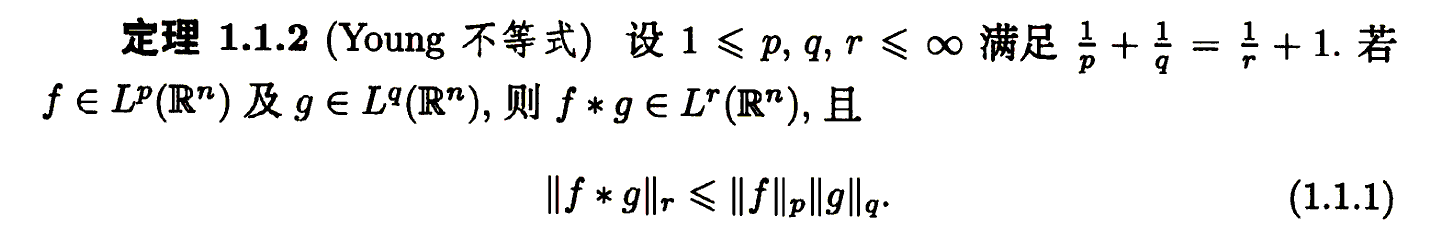
\includegraphics[width=\textwidth]{picture/young.PNG}
\end{framed}

\begin{framed}
\setlength{\parindent}{0pt}
[周民强, 实变函数论(第2版), p.186]
\vspace{0.1cm}
    
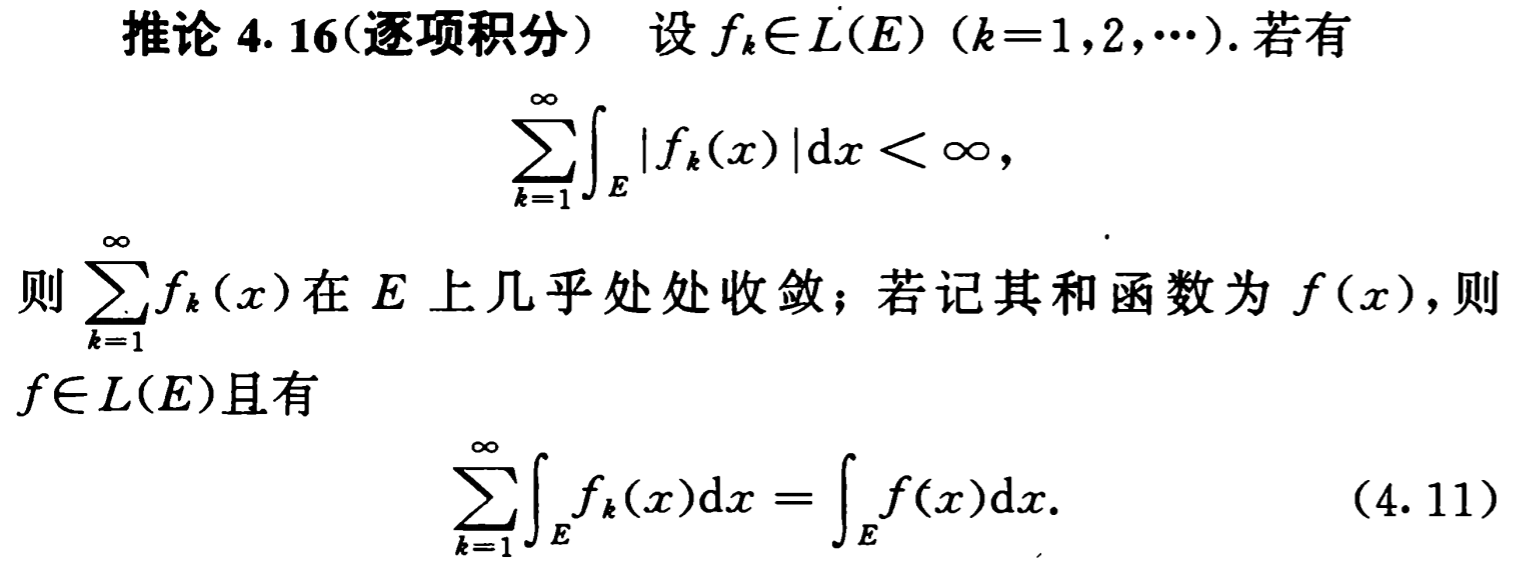
\includegraphics[width=\textwidth]{picture/add.PNG}
\end{framed}

\begin{framed}
\setlength{\parindent}{0pt}
[周民强, 实变函数论(第2版), p.139]
\vspace{0.1cm}
    

\includegraphics[width=\textwidth]{picture/riesz.PNG}
\end{framed}

\newpage

\begin{framed}
\setlength{\parindent}{0pt}
[伍胜健, 数学分析(第2册), p.107]
\vspace{0.1cm}
    
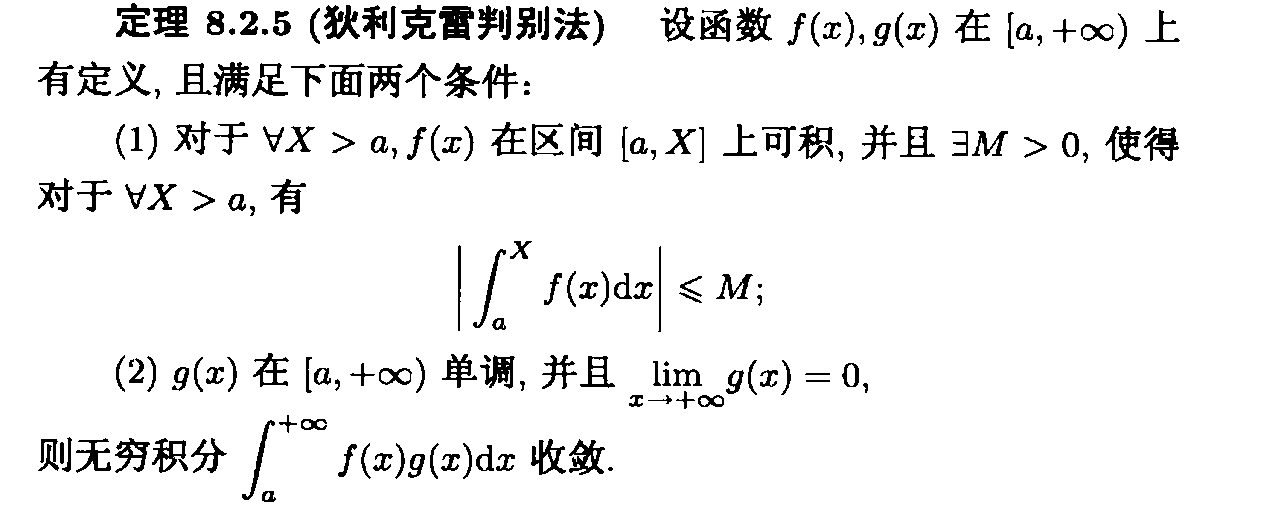
\includegraphics[width=\textwidth]{picture/dirichlet.PNG}
\end{framed}


\begin{framed}
\setlength{\parindent}{0pt}
[丁勇, 现代分析基础, p.50]
\vspace{0.1cm}


\includegraphics[width=\textwidth]{picture/convolution.PNG}
\end{framed}

\begin{framed}
\setlength{\parindent}{0pt}
[周民强, 实变函数论(第2版), p.326]
\vspace{0.1cm}

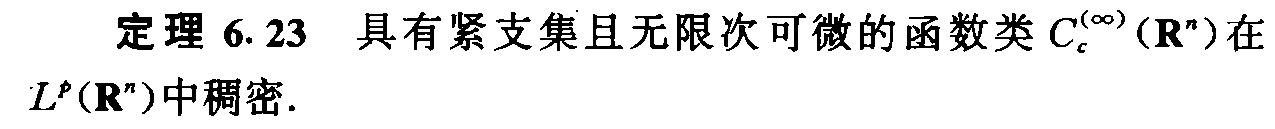
\includegraphics[width=\textwidth]{picture/dense.PNG}
\end{framed}

周民强定理中的 $ p \in [1, \infty) $. 
事实上, 孙镜淞证明了当 $ p \in (0, 1) $ 时,
$ C_c^\infty(\mathbb{R}) $ 同样在 $ L^p(\mathbb{R}) $ 中稠密.


\begin{framed}
\setlength{\parindent}{0pt}
[G. B. Folland, Real Analysis, p.188]
\vspace{0.1cm}

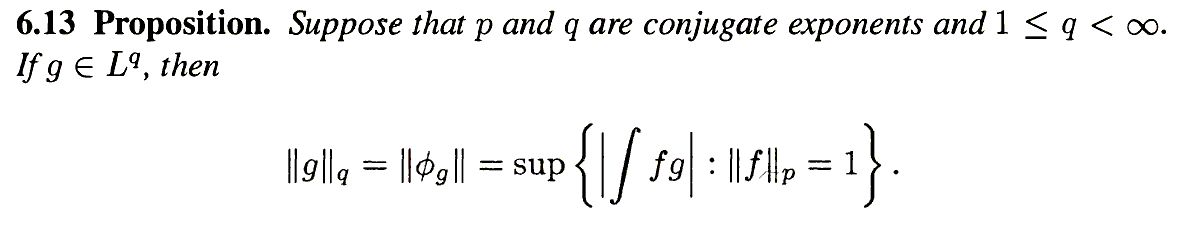
\includegraphics[width=\textwidth]{picture/dual.PNG}
\end{framed}


\end{document} 


